\documentclass[12pt,a4paper]{article}
\usepackage[italian]{babel}
\usepackage{newlfont}
\usepackage{float}
\usepackage{wrapfig}
\usepackage{natbib}
\usepackage{graphicx}
\usepackage{listings}
\usepackage{color}
\usepackage{hyperref}
\usepackage{xcolor}
\usepackage{listings}

\definecolor{mygray}{rgb}{0.5,0.5,0.5} 

\lstset{
	basicstyle=\footnotesize\ttfamily,
	keywords={typeof, new, true, false, catch, function, return, null, catch, switch, var, if, in, while, do, else, case, break},
  keywordstyle=\color{blue}\bfseries,
  ndkeywords={class, export, boolean, throw, implements, import, this},
  ndkeywordstyle=\color{darkgray}\bfseries,
  identifierstyle=\color{black},
  sensitive=false,
  comment=[l]{//},
  morecomment=[s]{/*}{*/},
  commentstyle=\color{mygray}\ttfamily,
  stringstyle=\color{red}\ttfamily,
  morestring=[b]',
  frame=L,
	breaklines=true,
	frameround=ffff,
	frame=L,
	tabsize=2,
	aboveskip=1em,
	belowskip=1em,
}

\hypersetup{
  colorlinks=true,
  linkcolor=black,
  citecolor=black,
  urlcolor=black,
  filecolor=black      
}


\renewcommand{\labelenumii}{\arabic{enumi}.\arabic{enumii}}
\renewcommand{\labelenumiii}{\arabic{enumi}.\arabic{enumii}.\arabic{enumiii}}
\renewcommand{\labelenumiv}{\arabic{enumi}.\arabic{enumii}.\arabic{enumiii}.\arabic{enumiv}}
  
\graphicspath{ {img/} }

\textwidth=450pt\oddsidemargin=0pt

\title{Lost 'n Souls} 
\author{Matteo Brocca, Alan Mancini, Federico Mazzini}
\date{Settembre 2021}\let\Date

\begin{document}
\begin{titlepage}
\begin{center}
	{{\Large{\textsc{Alma Mater Studiorum $\cdot$ Universit\`a di Bologna}}}} \rule[0.1cm]{15.8cm}{0.1mm}
	\rule[0.5cm]{15.8cm}{0.6mm}
	{\small{\bf Corso di\\Paradigmi di Programmazione e Sviluppo\\Docenti: Mirko Viroli, Roberto Casadei}}
\end{center}
\vspace{15mm}
\begin{center}
	{\Huge{\bf Lost 'n Souls}}\\
	\vspace{4mm}
	{\Huge{\bf Roguelike game}}
\end{center}
\vspace{40mm}
\par
\noindent
\begin{center}
{\large{
	\textit{Autori}:\\  
	Matteo Brocca $\cdot$ 1005681\\
	Alan Mancini $\cdot$ 1005481\\
	Federico Mazzini $\cdot$ 980559\\
}}
\end{center}
\vspace{40mm}
\begin{center}
	\large{Settembre 2021}
\end{center}
\end{titlepage}

\newpage

\tableofcontents
\newpage

\section*{Introduzione}
Il progetto scelto mira a sviluppare un single player game di genere Roguelike, 
ispirato al videogioco The Binding of Isaac.

Scopo del gioco, per un giocatore, è controllare un personaggio all’interno di un dungeon 
composto in modo procedurale da un numero finito di stanze definite in maniera procedurale. 
All’interno delle stanze saranno presenti in maniera casuale elementi bloccanti, nemici e oggetti. 
Il giocatore dovrà cercare di sconfiggere i nemici per passare alla stanza successiva e 
raccogliere oggetti al fine di potenziarsi o cambiare le sue caratteristiche. 
Una partita termina con la sconfitta del boss, un nemico unico presente all’interno del dungeon  in una specifica stanza, 
o con la morte perenne del personaggio, dove i progressi fatti durante il gioco vengono persi.
\addcontentsline{toc}{section}{Introduzione}
\section{Processo di sviluppo adottato}

% (modalità di divisione in itinere dei task, meeting/interazioni pianificate, modalità di revisione in itinere dei task, scelta degli strumenti di test/build/continuous integration)

Il processo di sviluppo adottato dal team è incrementale e iterativo. Si è cercato il più possibile di attenersi al framework \textbf{Scrum}, adattato alle esigenze lavorative e scolastiche dei membri del team. 
Il team ha effettuato \textbf{sprint} settimanali, in modo tale da massimizzare il numero di cicli iterativi di sviluppo. 
Inizialmente, gli sprint hanno avuto una parte di \textbf{planning}, mentre al loro termine, una parte di \textbf{review}.
Di seguito si analizza nel dettaglio il metodo utilizzato.

\subsection{Meeting}
Ai meeting ha sempre partecipato il team al completo. Al bisogno, Matteo ha svolto il ruolo di esperto di dominio/committente. Ogni scelta all'interno del progetto è comunque sempre stata condivisa da tutto il team. 
\subsubsection{Sprint planning}
Lo sprint planning è svolto all'inizio di ogni Sprint ed è di fondamentale importanta in quanto permette di definire nel dettaglio i task da eseguire all'interno dello sprint e i goal per esso.
Ogni sprint planning si compone di:
\begin{itemize}
    \item Raffinamento del product backlog e identificazione dei goal per lo sprint.
    \item Definizione dei \textbf{Task} come unità di lavoro pratica per soddisfare i \textbf{requisiti};
    \item Assegnazione dei Task ai membri del team.
\end{itemize}
Lo Sprint Planning ha una durata massima di 2 ore.

\subsubsection{Daily Scrum}
Durante il Daily Scrum ogni sviluppatore espone al team i seguenti punti:

\begin{itemize}
    \item Quale lavoro ha svolto la giornata precedente;
    \item Quale lavoro intende svolgere nella giornata corrente;
    \item Eventuali possibili impedimenti per il lavoro da svolgere, e come gli altri membri del team potrebbero aiutare ad affrontare il problema.
\end{itemize}
La durata di questo incontro è al massimo di 15 minuti.

\subsubsection{Sprint review}
La Sprint review analizza l'iterazione appena avvenuta e si concentra sul prodotto software in sè, in particolare si discute di:

\begin{itemize}
    \item Ispezione dell'incremento ottenuto in termini di funzionalità e risultati tangibili per il cliente
    \item Adattamento del Product Backlog;
    \item Discussione su ciò che potrebbe essere fatto nel prossimo Sprint, utile come pre\-pa\-ra\-zione al prossimo Sprint Planning.
\end{itemize}
Durata massima: 1 ora.

\subsubsection{Sprint retrospective}
La Sprint retrospective analizza l'iterazione appena avvenuta concentrandosi sul processo di sviluppo e il team, in particolare si discute di:

\begin{itemize}
    \item Come sono stati utilizzati i tool per il team e si analizza l'andamento dei meeting
    \item Idee per migliorare il processo di sviluppo, in particolare i punti critici individuati al punto sopra
\end{itemize}
Durata massima: 45 minuti.

\subsection{Divisione dei Task}

La suddivisione dei task è su base volontaria. Questo significa che tutti i membri del team si offrono volontariamente per svolgere un determinato task, nei limiti ovviamente della totalità dei task e dei goal per lo specifico sprint.
Durante il daily scrum, può essere rivista qualche decisione, se non troppo radicale.

\subsection{Definition of done}

Il team ha definito, come e in che modo, un task può essere definito come done e di conseguenza concluso
\begin{enumerate}
    \item Superamento di tutti gli Scalatest
    \item Codice documentato con opportuna Scaladoc
    \item Code review 
\end{enumerate}

\subsection{Tool}

Il team ha individuato i seguenti strumenti per favorire un processo agile, migliorare l'efficienza e favorire l'automazione durante il processo di sviluppo
\begin{itemize}
    \item \textbf{SBT} come strumento di build automation
    \item \textbf{Scalatest} per la scrittura ed esecuzione dei test automatizzati
    \item \textbf{GitHub} come strumento per la \textit{continuous integration}
    \item \textbf{Jira} come strumento a supporto di scrum, gestione del product backlog e delle varie board di sviluppo
\end{itemize}
\section{Requisiti}

\subsection{Requisiti di business}
%Requirement di alto livello stabiliscono perché si sta facendo 
%il sistema e quali siano i suoi vantaggi. 
\begin{itemize}
    \item Creazione di un gioco di genere Roguelike single player con la possibilità per un utente di comandare un personaggio all'interno di una mappa composta da stanze, affrontare nemici, raccogliere oggetti e sconfiggere un nemico finale.
    \item Possibilità di gioco su browser
\end{itemize}

\subsection{Requisiti utente}
%Quando un utente usa il sistema, cosa vuole fare e cosa si aspetta?
%Raccolgono le aspettative per un utente.
%Un modo tipico per documentare i requisiti utente sono le user stories.

Matteo Brocca in questo progetto ricopre il ruolo di esperto di dominio e committente. 
E' un appassionato di giochi Roguelike ma essendo troppo bravo li ha finiti tutti. 
Da qui l'idea di crearne uno nuovo per lui. 

\begin{enumerate}
    \item L'utente potrà 
    \begin{enumerate}
        \item avviare una nuova partita da un menu contestuale
        \item controllare con la tastiera il proprio personaggio all'interno della stanza per
        \begin{enumerate}
            \item spostarsi e cambiare direzione
            \item sparare ai nemici che possono essere di diversa tipologia
            \item evitare elementi bloccanti o di disturbo se presenti
            \item raccogliere oggetti utili all'aumento delle sue caratteristiche
            \item spostarsi da una stanza all'altra attraverso delle porte
        \end{enumerate}
        \item visualizzare in modo continuo le sue statistiche e i suoi punti vita
        \item visualizzare in modo continuo una mappa del dungeon che indichi la sua posizione corrente
       
    \end{enumerate}
    \item L'utente dovrà riuscire a 
    \begin{enumerate}
        \item distinguere visivamente nemici, oggetti e elementi di disturbo
        \item capire in che direzione si sta muovendo
        \item capire dove sta sparando
        \item capire di aver colpito un nemico
        \item capire di aver raccolto un oggetto
        \item capire qual'è la stanza del boss
        \item capire che sta fronteggiando un boss
        \item capire di aver vinto o perso una partita
    \end{enumerate}
\end{enumerate}

\subsection{Requisiti funzionali}
%Funzionali: statement dettagliati delle funzionalità del sistema indicate
%in modo chiaro (organizzarli permette uno sviluppo del progetto rigoroso)
\begin{enumerate}
    \item Menù di gioco
    \begin{enumerate}
        \item presenza di un tasto per avviare una nuova partita
    \end{enumerate}
    \item Caricamento del gioco
    \begin{enumerate}
        \item presenza di una schermata durante il caricamento degli elementi di gioco
    \end{enumerate}
    \item Generazione del dungeon/mappa di gioco 2D in maniera casuale
    \begin{enumerate}
        \item Durante la generazione deve essere visualizzata una schermata di attesa
        \item Un dungeon è formato da più stanze quadrate
        \item Ogni stanza è fisicamente adiacente ad almeno un'altra stanza
        \item Tra stanze adiacenti è presente una porta che le collega
        \item La disposione delle stanze avviene favorendo forme di mappa complesse simil labirinto 
        \item Una stanza è di una tipologia fra
            \begin{enumerate}
                \item Vuota
                    \begin{enumerate}
                        \item Stanza completamente vuota
                        \item La partita comincia con il personaggio in una stanza vuota
                        \item In un dungeon ci sono circa un 10\% di stanze vuote
                    \end{enumerate}
                \item Oggetto
                    \begin{enumerate}
                        \item Contiene al centro un singolo oggetto scelto randomicamente
                        \item In un dungeon ci sono circa un 15\% di stanze oggetto
                    \end{enumerate}
                \item Combattimento
                    \begin{enumerate}
                        \item Il contenuto è generato randomicamente
                        \item Contiene alcuni nemici
                        \item Contiene alcuni elementi bloccanti disposti in modo da non ostruire l'accesso alle porte da parte del personaggio
                        \item Le porte si chiudono quando il giocatore entra nella stanza
                        \item Le porte si aprono quando il giocatore ha eliminato tutti i nemici
                        \item In un dungeon ci sono circa un 75\% di stanze combattimento
                    \end{enumerate}
                \item Boss
                    \begin{enumerate}
                        \item Contiene solamente il nemico boss
                        \item Una sola nel dungeon
                        \item Adiacente ad una ed una sola altra stanza
                    \end{enumerate}
            \end{enumerate}
        
        
    \end{enumerate}

    \item Scena di gioco
    \begin{enumerate}
        \item A video, dopo la generazione del dungeon, è visibile
        \begin{enumerate}
            \item al centro dello schermo e rappresentata con vista dall'alto solo la stanza dove è correntemente presente il personaggio
            \item a sinistra della stanza l'elenco delle statistiche del personaggio
            \item a sinistra della stanza una mini mappa del dungeon
            \begin{enumerate}
                \item Le stanze vuote e combattimento sono di colore neutro (bianco)
                \item La stanza corrente, quelle oggetto e la stanza boss sono evidenziate con colori propri 
            \end{enumerate}
        \end{enumerate}
        \item All'interno di una stanza nemici, oggetti, elementi bloccanti e personaggio, in linea generale
            \begin{enumerate}
                \item sono vincolati a stare nei limiti del perimetro rappresentato dal pavimento
                \item non possono fisicamente attraversarsi tra loro sovrapponendosi graficamente, tuttavia la parte in alto di un'entità può sovrapporsi alla parte bassa di un'altra senza generare collisione ad emulare altezze diverse
            \end{enumerate}
        \item All'interno di una stanza un colpo sparato
        \begin{enumerate}
            \item è rappresentato con un cerchio colorato
            \item è vincolato a stare nei limiti del perimetro rappresentato dal pavimento
            \item colpisce un'entità qualsiasi non appena il primo entra in contatto con il rettangolo che graficamente racchiude interamente la seconda 
            \item quando colpisce qualcosa il cerchio viene sostituito da un esplosione animata
        \end{enumerate}
        
    \end{enumerate}
    
    \item Personaggio controllabile con caratteristiche e punti vita
    \begin{enumerate}
        \item Il personaggio è caratterizzato da
            \begin{enumerate}
                \item Punti vita
                \item Tempo invulnerabilità dopo essere stato colpito
                \item Velocità di movimento
                \item Rate dello sparo
                \item Danno dei proiettili
                \item Velocità dei proiettili
                \item Range dei proiettili
            \end{enumerate}
        \item Il personaggio è controllato dall'utente con la tastiera
        \begin{enumerate}
            \item L'utente può muovere il personaggio nelle quattro direzioni principali (sopra, sotto, destra, sinistra)
            \item L'utente può sparare uno o più colpi verso una delle quattro direzioni principali (sopra, sotto, destra, sinistra)
            \item Il personaggio può uscire dalla stanza attraverso le porte
        \end{enumerate}
        \item Il personaggio è visivamente costituito da
        \begin{enumerate}
            \item Una testa orientata in modo da rappresentare la direzione di fuoco, se il personaggio non sta sparando allora è orientata nella direzione di movimento
            \item Un corpo orientato ed animato in modo da rappresentare la direzione di movimento
        \end{enumerate}
        \item Il personaggio infligge danno ai nemici quando un suo colpo colpisce un nemico
        \item Il personaggio può raccogliere oggetti che modificano le sue caratteristiche
        \item Il personaggio muore e la partita termina mostrando un messaggio "game over" quando la sua vita arriva a zero
    \end{enumerate}
    
    \item Nemici con diverse caratteristiche e comportamenti
    \begin{enumerate}
        \item Un nemico può essere nello stato
        \begin{enumerate}
            \item Inattivo: non esegue azioni
            \item Attacco: esegue azioni di attacco nei confronti del personaggio
            \item Difesa: esegue azioni per difendersi dal personaggio
            \item Nascosto: esegue azioni per nascondersi dal personaggio
        \end{enumerate}
        \item Ogni nemico è caratterizzato da
            \begin{enumerate}
                \item Punti vita
                \item Velocità di movimento
                \item Danno da contatto
                \item Se il nemico spara
                \begin{enumerate}
					\item Rate dello sparo
					\item Danno dei proiettili
					\item Velocità dei proiettili
					\item Range dei proiettili
                \end{enumerate}
            \end{enumerate}
        \item Un nemico infligge danno al personaggio quando vi entra in collisione
        \item Un nemico che spara infligge danno al personaggio quando un suo colpo vi entra in collisione
        \item Un nemico se si muove lo fa solo all'interno di una sola stanza
        \item Un nemico muore quando la sua vita arriva a zero, al suo posto viene visualizzata un esplosione animata
        \item Quattro tipologie di nemico
            \begin{enumerate}
                \item Nerve
                    \begin{enumerate}
                        \item Sta sempre nello stato di attacco
                        \item Sta immobile
                        \item Costituito da un corpo
                    \end{enumerate}
                \item Boney
                    \begin{enumerate}
                        \item Sta sempre nello stato di attacco
                        \item Si sposta continuamente in direzione del personaggio
                        \item Costituito da testa e corpo orientati nella direzione di movimento
                    \end{enumerate}
                \item Mask
                    \begin{enumerate}
                        \item Sta sempre nello stato di attacco
                        \item Si sposta mantenendo una distanza predefinita dal personaggio
                        \item Spara colpi in direzione del personaggio
                        \item Costituito da una testa orientata nella direzione di fuoco
                    \end{enumerate}
                \item Parabite
                    \begin{enumerate}
                        \item Sta 1 secondo nello stato "inattivo", poi passa allo stato di "attacco", poi allo stato "nascosto" per 2 secondi poi ricomincia da capo
                        \item Quando passa da inattivo ad attacco calcola una linea retta in direzione del personaggio e la percorre velocemente
                        \item Quando passa allo stato "nascosto" può essere attraversato da personaggio o altri nemici e non può essere colpito
                        \item Costituito da un corpo orientato nella direzione di movimento
                    \end{enumerate}
            \end{enumerate}
        \item Boss
        \begin{enumerate}
            \item E' un nemico speciale che se viene sconfitto la partita termina visualizzando al giocatore il messaggio "hai vinto"
            \item Il suo comportamento è determinato da 5 diverse azioni scelte casualmente con una certa probabilità in base al suo stato di vita e quello del personaggio.
            \begin{enumerate}
				\item Attacco con singolo proiettile in direzione del personaggio se questo si trova sullo stesso asse x o y all'interno della stanza
				\item Attacco che spara 4 proiettili in contemporanea: sopra, sotto, destra e sinistra
				\item Attacco che spara 4 proiettili in contemporanea in diagonale: sopra, sotto, destra e sinistra
				\item Si sposta verso il personaggio per aggredirlo
				\item Si teletrasporta in un punto della stanza specchiato rispetto a quello attuale. Se il punto è occupato da un elemento bloccante, trova il primo posto libero nel suo intorno
			\end{enumerate}
            \item Costituito da un corpo
        \end{enumerate}
    \end{enumerate}
    
    \item 10 Oggetti che il personaggio può raccogliere per incrementare le proprie caratteristiche
    \begin{enumerate}
        \item Arrow: incermenta il rate dello sparo 
        \item Drop: incermenta il danno dei proiettili
        \item Eye: incrementa il danno dei proiettili ed il rate dello sparo
        \item Fireball: incrementa il danno e la velocità dei proiettili
        \item Glasses: incrementa il range dei proiettili
        \item Heart: incrementa la vita massima di 1
        \item Juice: incrementa la velocità di spostamento e danno del fuoco
        \item Mushroom: incrementa la vita massima di 2
		\item Syringe: incrementa la velocità di spostamento, il rate dell sparo e la velocità dei proiettili
		\item Tail: incrementa il danno ed il range dei proiettili
    \end{enumerate}
         
\end{enumerate}


\subsection{Requisiti non funzionali}
%Non funzionali: statement dettagliati che raccolgono la qualità del 
%comportamento o sui vincoli del sistema

\begin{enumerate}
    \item Fluidità di gioco
    \begin{enumerate}
        \item Deve essere garantita una velocita di almeno 30 FPS su processore Apple M1 in situazioni di gioco "caotiche", dove per caotico si intende la presenza all'interno di una stanza del Character comandato dal giocatore, 5 nemici, 10 shot e 10 elementi bloccanti.
    \end{enumerate}
\end{enumerate}


\subsection{Requisiti di implementazione}
%Implementazione: requirement posti agli sviluppatori. Danno indicazioni 
%sul lavoro da fare. Possono comprendere: tipi di strumenti utilizzati, 
%modi di sviluppo, documentazione fornita.

\begin{enumerate}
\item Implementazione mediante Scala 3
\item Implementazione mediante Prolog della generazione del dungeon, delle stanze combattimento e del comportamento del Boss
\item Testing mediante ScalaTest
\item Sviluppo del software in modo da considerare possibili future estensioni di gioco come:
\begin{enumerate}
    \item Aggiunta di diversi personaggi con cui giocatore
    \item Aggiunta di nuovi nemici e boss
    \item Aggiunta di nuovi elementi bloccanti
    \item Aggiunta di nuovi oggetti con diverse caratteristiche
\end{enumerate}
\item Rilascio del gioco su server tramite GitHub Actions
\end{enumerate}
\section{Design architetturale}
%Design architetturale (architettura complessiva, descrizione di pattern architetturali usati, componenti del sistema distribuito, scelte tecnologiche cruciali ai fini architetturali -- corredato da pochi ma efficaci diagrammi)

Di seguito vengono analizzate l'architettura complessiva dell'applicazione e le decisioni critiche riguardanti pattern architetturali e tecnologie rilevanti.
Prima di pensare a qualsiasi architettura per il gioco da realizzare, ciò che si è cercato di fare è stato individuare l'engine ideale per il progetto. 
La scelta è ricaduta su Indigo in quanto: 
\begin{itemize}
    \item E' un framework specifico per il game development
    \item E' scritto in Scala 3 e favorisce lo sviluppo tramite paradigma funzionale con un approccio unidirezionale ed immutabile al flusso di dati
    \item Permette il gioco su browser, come da requisito di business, mediante compilazione tramite Scala.js.
\end{itemize}
I concetti chiave di Indigo che ci guidano nello sviluppo del gioco sono 
\begin{itemize}
    \item Paradigma Model, View, ViewModel
    \item Game loop con modello ad eventi
    \item Scene
\end{itemize}

\subsection{Paradigma Model-View-ViewModel}
Il pattern architetturale \textbf{MVVM} (Model, View, ViewModel) è una variante del famoso MVC. 
Obiettivo di questo pattern è quello di separare il modello dei dati dalla sua rappresentazione, tenendo entrambi puri e funzionali al loro scopo, frapponendo tra loro un elemento "ibrido", il ViewModel.
Di seguito l'interpretazione sulla quale si basa Indigo e che seguiamo per lo sviluppo del nostro gioco.


\begin{figure}[!hbt]
    \centering
    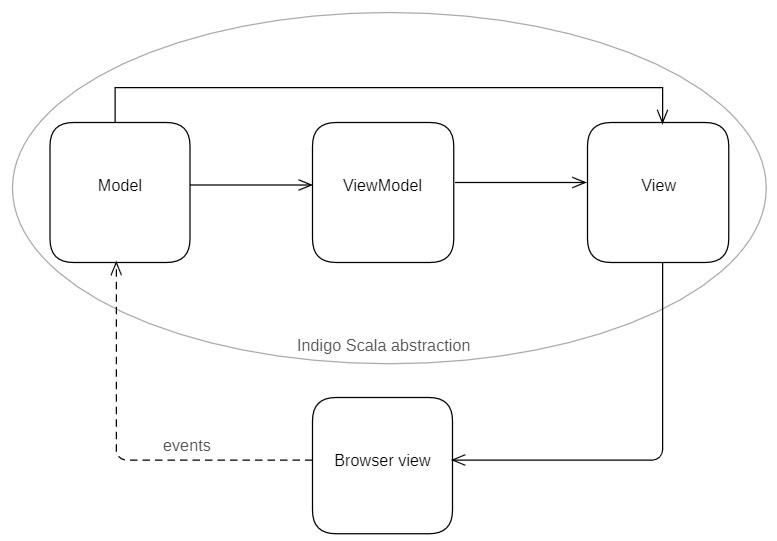
\includegraphics[scale=0.5]{mvvm.jpg}
    \caption{\textit{Architettura Model, View, ViewModel}} 
\end{figure}

\paragraph{Model}
Rappresenta il modello di gioco puro, indipendentemente dalla sua rappresentazione visuale. 
Esso contiene lo stato del gioco e la sua logica. 

\paragraph{ViewModel}
Si interpone tra Model e View. Ha lo scopo di mantenere alcuni dati utili per la rappresentazione che tuttavia non concernono la logica di gioco, devono perciò rimanere separati e non essere inclusi all'interno del Model.

\paragraph{View}
Si occupa di offrire una rappresentazione del Model e del ViewModel a schermo. Costituisce quindi la logica di visualizzazione di questi, senza contenere però alcuno stato o logica di gioco.

\subsection{Game loop con modello ad eventi}
La logica di Indigo si basa su un game loop che processa, ad ogni iterazione, una coda di eventi. 
Ad ogni ciclo, il framework esegue le seguenti operazioni:
\begin{itemize}
    \item Aggiunta dell'evento FrameTick alla coda eventi
    \item Per ogni evento, update del Model
    \item Per ogni evento, update del ViewModel
    \item Presentazione e rendering degli elementi a video
    \item Reset della coda di eventi
\end{itemize}

Il concetto di \textbf{immutabilità}, presente nel paradigma funzionale, qui si traduce non in un update di uno stato interno del modello, ma bensì nella generazione di un nuovo modello aggiornato. 

Durante l'update del Model è possibile generare eventi custom che verranno processati all'iterazione successiva: a tale scopo Indigo fornisce la \textbf{monade Outcome} utile a wrappare dati ed eventi. 

\subsection{Scene}
Le scene sono un modo di organizzare il codice secondo una logica di gioco ben definita. Sono un meccanismo di suddivisione che permette di individuare delle "fasi" di gioco da sviluppare in modo separato le une dalle altre.
In ogni istante all'interno del gioco la scena indicata come "corrente" è abilitata all'aggiornamento del Model/ViewModel, alla gestione degli eventi in coda ed infine alla presentazione a schermo: la scena corrente può leggere e aggiornare solo i suoi dati che sono un sottoinsieme di quelli globali. 

Abbiamo identificato quattro scene principali su cui andare a definire Lost 'n Souls. 

\begin{figure}[!hbt]
    \centering
    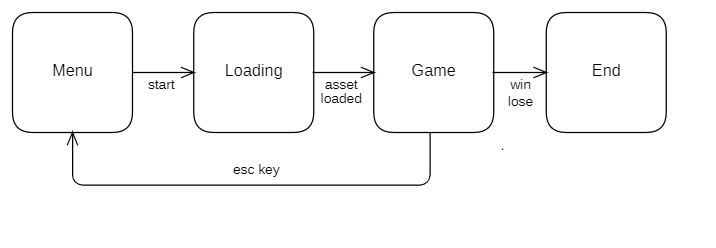
\includegraphics[scale=0.75]{scenes.jpg}
    \caption{\textit{Il flusso delle scene}}
\end{figure}

\subsection{Architettutra di Model e ViewModel}

Come conseguenza della suddivisione di cui sopra, il Model principale è costituito dai singoli Model relativi a ciascuna scena. Stessa cosa vale per il ViewModel. 

Da notare che una scena, per la sua presentazione a video, può non necessitare di un Model o di un ViewModel, lo stesso concetto si può estendere per una View qualsiasi la quale potrebbe basarsi solo su Model.

\begin{figure}[!hbt]
    \centering
    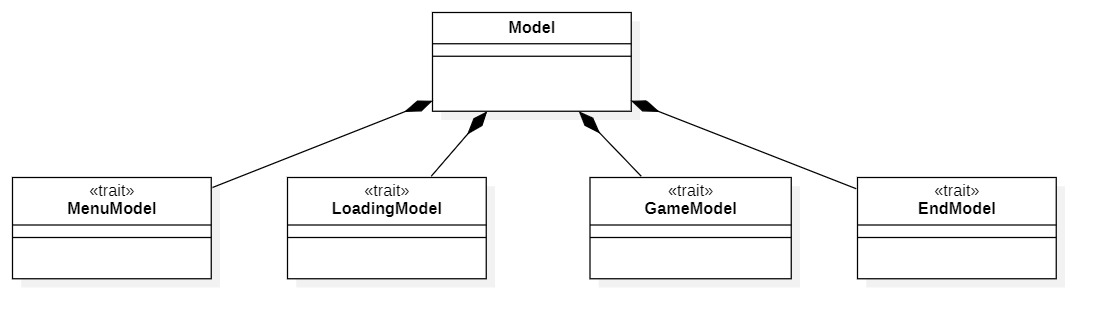
\includegraphics[scale=0.45]{model.jpg}
    \caption{\textit{Il Model}} 
\end{figure}

\newpage 
\subsection{Elementi principali del GameModel}
All'interno della scena di gioco, abbiamo identificato i principali componenti:

\begin{itemize}
    \item \textbf{Character} Personaggio controllato dal giocatore
    \item \textbf{Dungeon} Intera mappa di gioco nel suo complesso
    \item \textbf{Room} Stanza situata all'interno di una mappa di gioco
    \item \textbf{Anything} Una qualsiasi entità da visualizzare all'interno di una stanza: nemico, oggetto, elemento bloccante o anche lo stesso Character. 
    
\end{itemize}


\begin{figure}[!hbt]
    \centering
    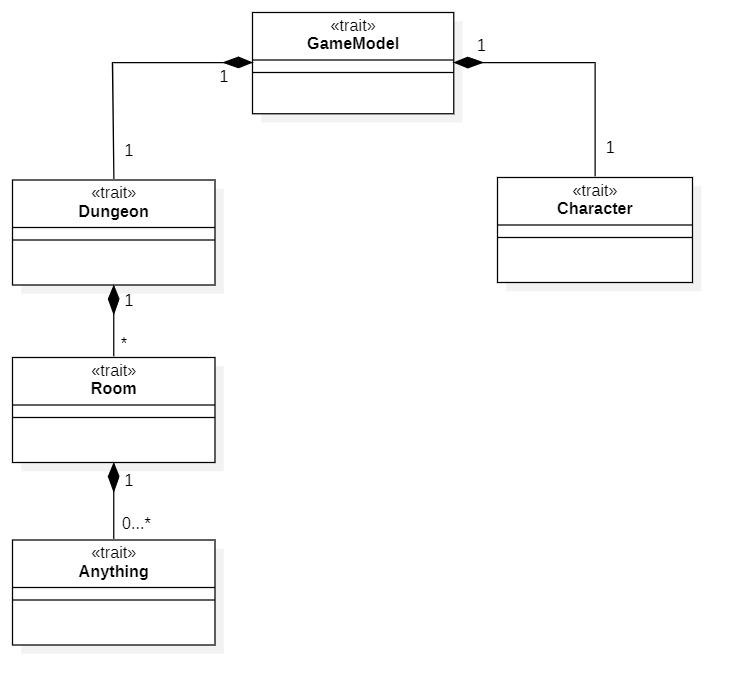
\includegraphics[scale=0.5]{gamemodel.jpg}
    \caption{\textit{Diagramma degli elementi principali del GameModel}} 
\end{figure}

\subsection{Anything OOP anziché pattern ECS}
Per concludere la descrizione dell'architettura occorre specificare come organizzare gli oggetti presenti nel gioco, quelli che abbiamo chiamato \textbf{Anything}.
Un oggetto è caratterizzato da proprietà e comportamenti comuni ad altri, ad esempio tutti gli oggetti sono posizionabili nella stanza di gioco e visualizzabili mentre alcuni di questi possono spostarsi, collidere, causare danno e così via.

Tradizionalmente molto usato nel game development è il pattern Entities-Components-Systems che prevede la sostituzione di una gerarchia di oggetti con il concetto di entità e componenti: le entità sono definite dai diversi componenti a loro associati. 
Alcune implementazioni di ECS definiscono i componenti come solo strutture dati mentre il comportamento è specificato nel sistema che li gestisce, quindi in stile funzionale. 
Questo pattern è nato per diversi motivi ma quello più banale è che, quando i linguaggi non supportano l'ereditarietà multipla, è impossibile specificare una precisa gerarchia di oggetti che soddisfi i requisiti di un gioco di una certa complessità, o comunque questa gerarchia sarebbe molto profonda e poco flessibile a future estensioni.

Quello che vogliamo fare in questo progetto è sfruttare appieno le potenzialità in ambito \textbf{OOP} che ci offre Scala, il quale ci permette tramite i \textbf{mix-ins} di appiattire la gerarchia ed ottenere la flessibilità richiesta dal problema.
Quindi abbiamo appositamente scelto il nome Anything in sostituzione al classico Entity per specificare che non stiamo applicando il pattern ECS, un sottotipo di Anything rappresenta una nostra entità che può essere mixata con altri tratti per ottenere nuove proprietà e comportamenti. 

Visto l'impiego del pattern MVVM, occorre inoltre tenere ben presente che un Anything deve essere in realtà codificato in tre parti ben distinte Model-ViewModel-View ciascuna sottotipo rispettivamente di \textbf{AnythingModel}, \textbf{AnythingViewModel} e \textbf{AnythingView} e ciascuna eventualmente mixata come descritto precedentemente. 
Inoltre è da specificare che ogni oggetto in gioco è costitutito sempre da un Model e una View ma quest'ultima potrebbe non necessitare di un ViewModel.

Il Model di un oggetto come comportamento base deve reagire alle richieste di aggiornamento che avvengono ad ogni iterazione del game loop: questa richiesta deve essere propagata a tutta la catena di ereditarietà e ai vari oggetti mixati ed infine restituire un nuovo Model aggiornato.
Sebbene gran parte del comportamento e della logica di gioco è così incapsulata nei Model degli oggetti, dovremmo comunque elaborare dei sistemi che avranno una visione globale gestendo l'interazione tra diversi Model, come un sistema per controllare le collisioni tra oggetti.

Per concludere, la nostra soluzione OO non è la migliore soluzione possibile per lo sviluppo di un gioco. Il pattern ECS ha vantaggi prestazionali riconosciuti sia in termini di utilizzo CPU (meno calls per l'aggiornamento degli oggetti) che di ottimizzazione dell'utilizzo della memoria (data-oriented design), tuttavia a fini didattici vogliamo sperimentare elementi di Scala OOP avanzati.

\subsection{Prolog engine e PrologService}
Il motore Prolog da utilizzare per la generazione del dungeon, delle stanze combattimento e del comportamento del Boss deve potersi integrare ed interagire con Indigo.
Poichè Indigo compila con Scala.js e per evitare possibili problemi con engine scritti in Java/Scala, la scelta di quale motore Prolog usare ricade su \textbf{TauProlog}, un engine scritto in Javascript e quindi facilmente integrabile nel nostro contesto.

Tuttavia per comunicare con questo motore occorre utilizzare la \textbf{programmazione asincrona} in quanto è strutturato in modo da rispondere alle interrogazioni mediante una \textbf{callback} che deve essere fornita.
Questa modalità di interazione non è supportata direttamente da Indigo, il quale con il suo game loop supporta come input eventi/messaggi che però possono essere generati solo internamente durante le fasi di update del Model: l'attivazione di una callback asyncrona fuori dal game loop non può ne modificare lo stato del Model che è immutabile ne generare un evento.

Per questo si rende necessario lo sviluppo di un componente separato che faccia da proxy per l'engine TauProlog e risponda alle richieste del gioco con opportuni eventi customizzati.

Indigo dispone dei \textbf{SubSystems}, servizi con un proprio Model ed esterni alla logica di gioco ma che vengono attivati nel game loop per intercettare eventi ed eseguire azioni: occorre quindi predispore un \textbf{PrologService} subsystem.

\begin{figure}[!hbt]
    \centering
    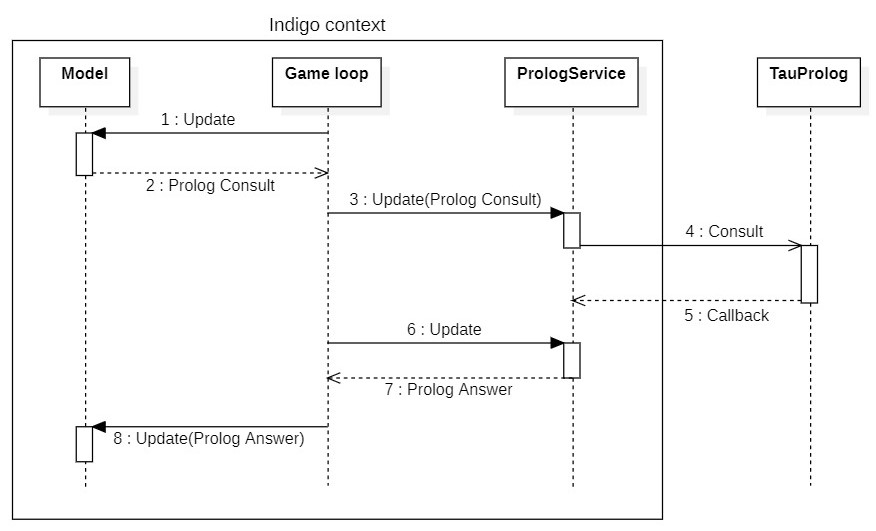
\includegraphics[scale=0.7]{prolog.jpg}
    \caption{\textit{Diagramma dell'interazione con TauProlog}} 
\end{figure}

In figura sotto è mostrata l'interazione tra i sistemi: da notare che la callback chiamata da TauProlog necessita di scrivere dati nel Model del PrologService invalidando così il concetto di immutabilità, ma solo per quel servizio esterno al gioco ed il tutto senza introdurre alcun problema di concorrenza in quanto ogni esecuzione di procedura è atomica nel contesto dell'\textbf{event loop} di Javascript.



\section{Design di dettaglio}
Design di dettaglio (scelte rilevanti, pattern di progettazione, organizzazione del codice -- corredato da pochi ma efficaci diagrammi)
Di seguito verranno analizzate le scelte di design rilevanti per il sistema, i pattern di progettazione utilizzati e l'organizzazione del codice. 
\subsection{GameModel}
L'intero modello di gioco, dallo stato al comportamento, è incapsulato all'interno della struttura GameModel. E' possibile identificare due diverse accezioni del modello, a seconda del momento di gioco. 
Un momento in cui la partita non è ancora stata avviata e un momento successivo in cui invece la partita è avviata.
Nel primo momento, a partita non avviata, è necessario generare il dungeon e le stanze che lo compongono. Nel secondo momento, una volta che è avvenuta la generazione, il modello è costituito da un Dungeon, composto da diverse stanze, e dal character controllato dal giocatore. 

\begin{figure}[!hbt]
    \centering
    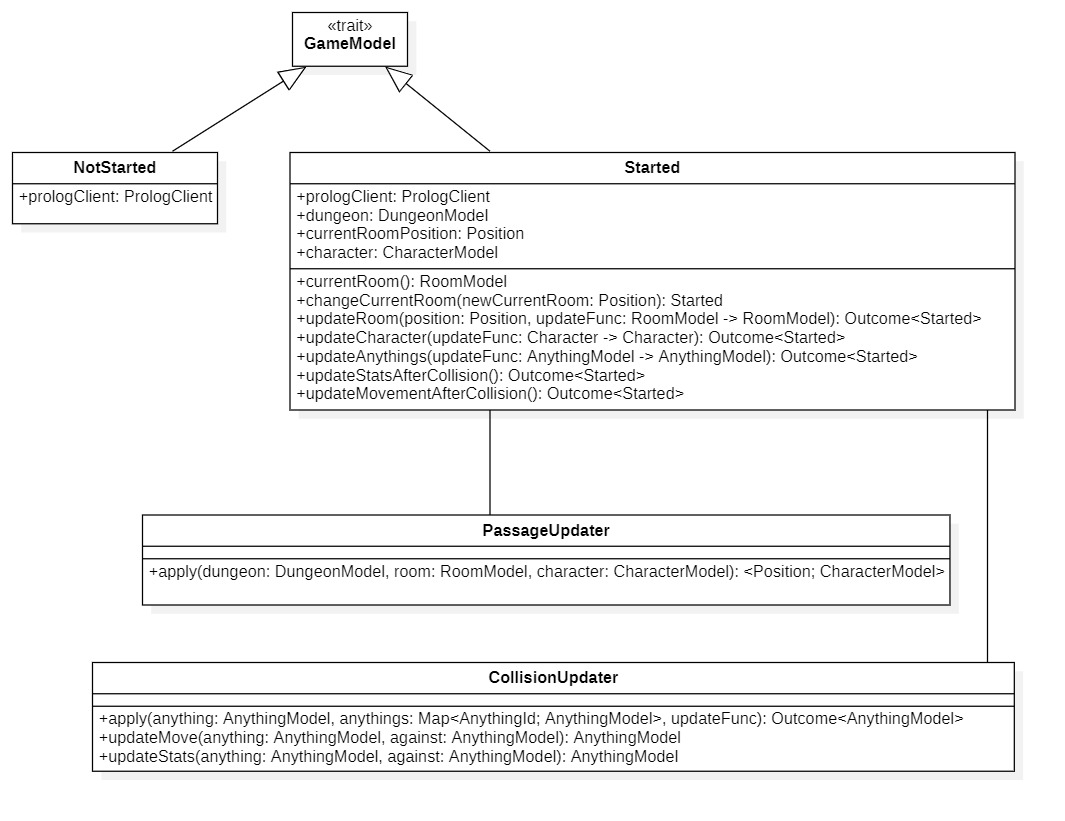
\includegraphics[scale=0.2]{GameModelClassDiagram.jpg}
    \caption{\textit{Game model class diagram (da modificare con versione pro di staruml)}} 
\end{figure}
Il modello di gioco rappresenta un'istantanea delle varie componenti che lo compongono in un determinato momento. 
Ogni modifica al modello consiste nella creazione di un nuovo modello con il componente aggiornato. 

Una scelta rilevante ai fini dell'implementazione è il fatto che, a livello di modello, il character controllato dal giocatore è sempre fuori dalla stanza in cui si trova, in questo modo è possibile aggiornare in maniera indipendente le due componenti.
\subsection{Dungeon}
Il dungeon è composto da stanze disposte in maniera randomica ma collegate tra loro. 
La struttura Grid è ciò che descrive un Dungeon nella sua forma più basilare e geometrica e offre delle operazioni per esplorarlo. 
\begin{figure}[!hbt]
    \centering
    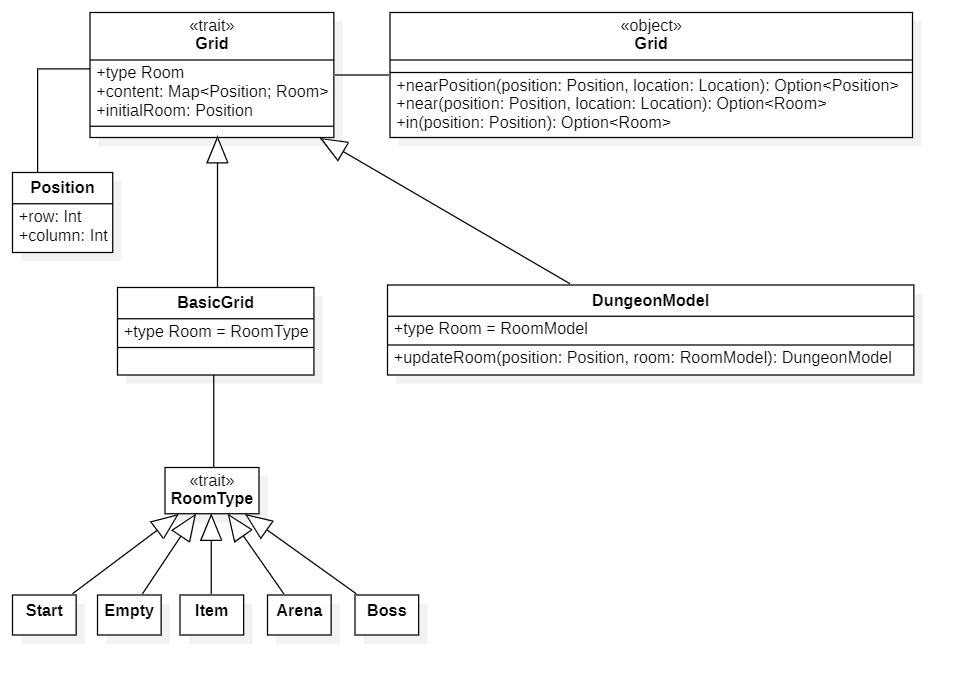
\includegraphics[scale=0.2]{DungeonClassDiagram.jpg}
    \caption{\textit{Dungeon class diagram(da modificare con versione pro di staruml)}} 
\end{figure}

Grid definisce quindi una collezione di stanze, di tipo ancora non definito, in una specifica posizione all'interno di una griglia di dimensioni \textit{n}. La definizione del tipo Room è lasciato alle specializzazioni di Grid, si mette quindi in pratica il pattern \textbf{Family Polimorfism}.

All'interno di una griglia, un elemento potrebbe o non potrebbe essere presente, andando così a definire un dungeon con stanze in posizioni diverse. 
E' necessario perciò lavorare con strutture dati che consentano l'assenza di un dato.

Il Dungeon vero e proprio prende forma quando il tipo Room viene definito con un modello consono a descriverne lo stato e il comportamento. 

\subsection{Room}
Come da requisiti, una stanza è la componente principale del Dungeon e può essere di diversi tipi: Empty, Arena, Item e Boss. 
Ogni stanza incapsula al suo interno gli elementi che sono rilegati all'interno e non possono muoversi all'interno del Dungeon, come ad esempio i nemici o gli elementi bloccanti. 

\begin{figure}[!hbt]
    \centering
    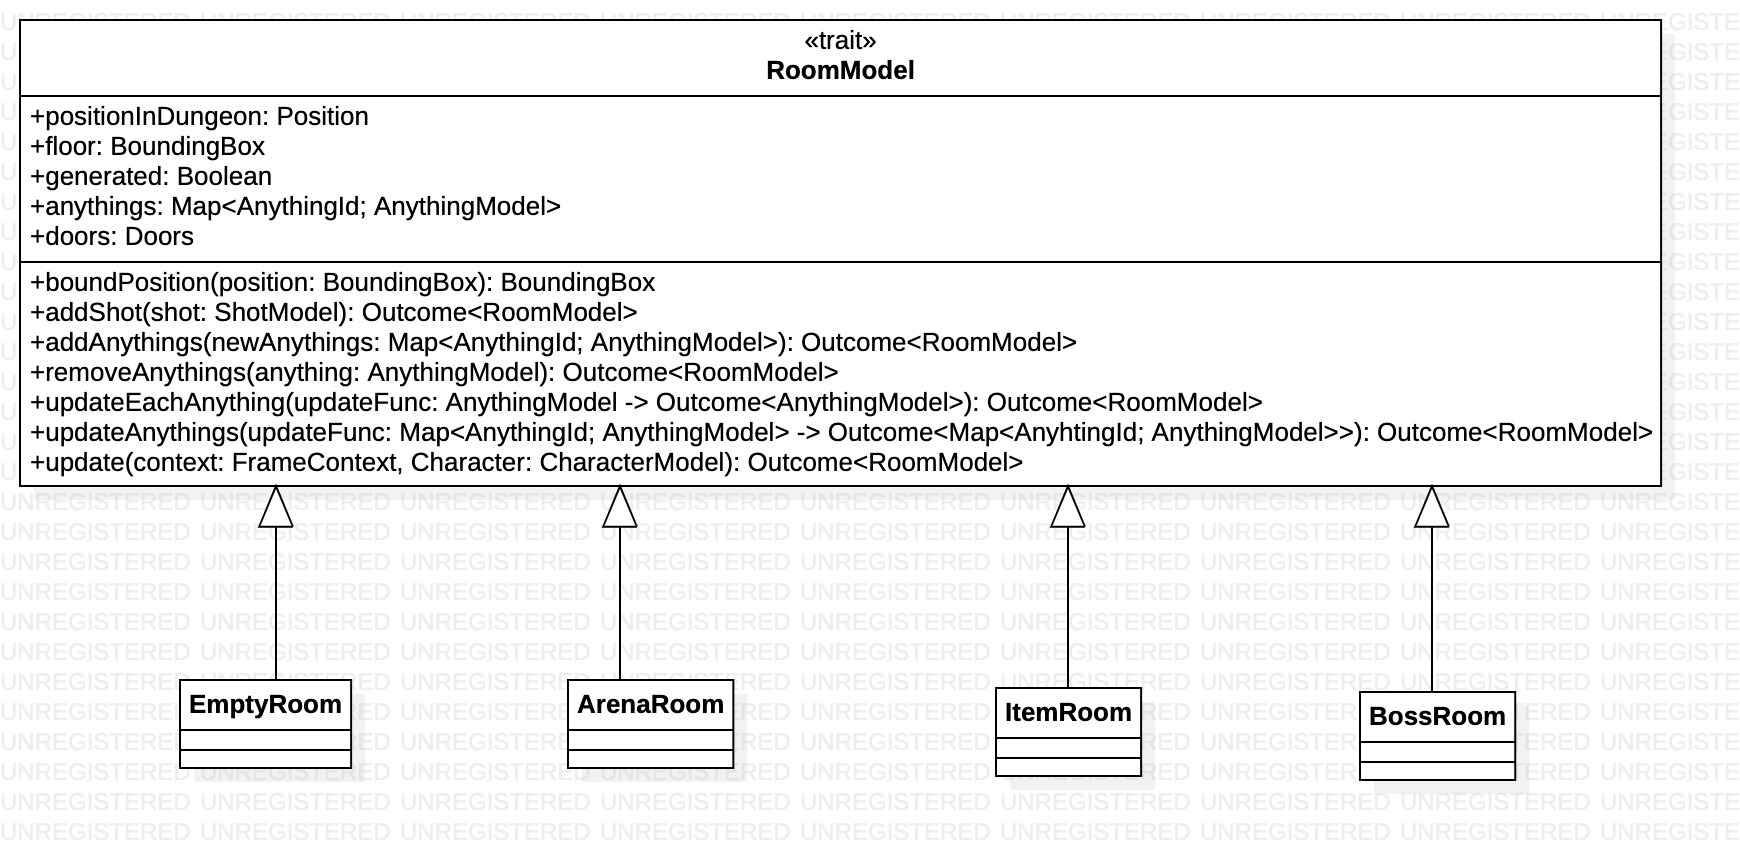
\includegraphics[scale=0.25]{RoomClassDiagram.jpg}
    \caption{\textit{Room class diagram(da modificare con versione pro di staruml)}} 
\end{figure}

Una stanza è anche responsabile dell'aggiornamento di tutto ciò che incapsula. Anche in questo caso si cerca di lavorare con strutture dati immutabili, perciò l'aggiornamento di uno o più componenti consegue una nuova stanza aggiornata. 
L'aggiornamento viene fatto ad ogni FrameTick ed è comandato dal dungeon, solamente per la stanza correntemente visualizzata, le altre stanze non sono aggiornate o gestite.  

\subsubsection{Door}
Un dettaglio importante di una stanza sono le porte che la collegano con altre stanze. Si è scelto di definire una porta non tanto come un link, ma come una proprietà statica, lasciando al Dungeon il compito di gestire il collegamento. 
Una porta è quindi l'associazione di un lato della stanza con lo stato della stessa. Il fatto che vi sia una porta, presuppone comunque che dalla parte opposta vi sia un'altra stanza, ma questo dettaglio è trasparente alla stanza e gestita dal Dungeon. 
\begin{figure}[!hbt]
    \centering
    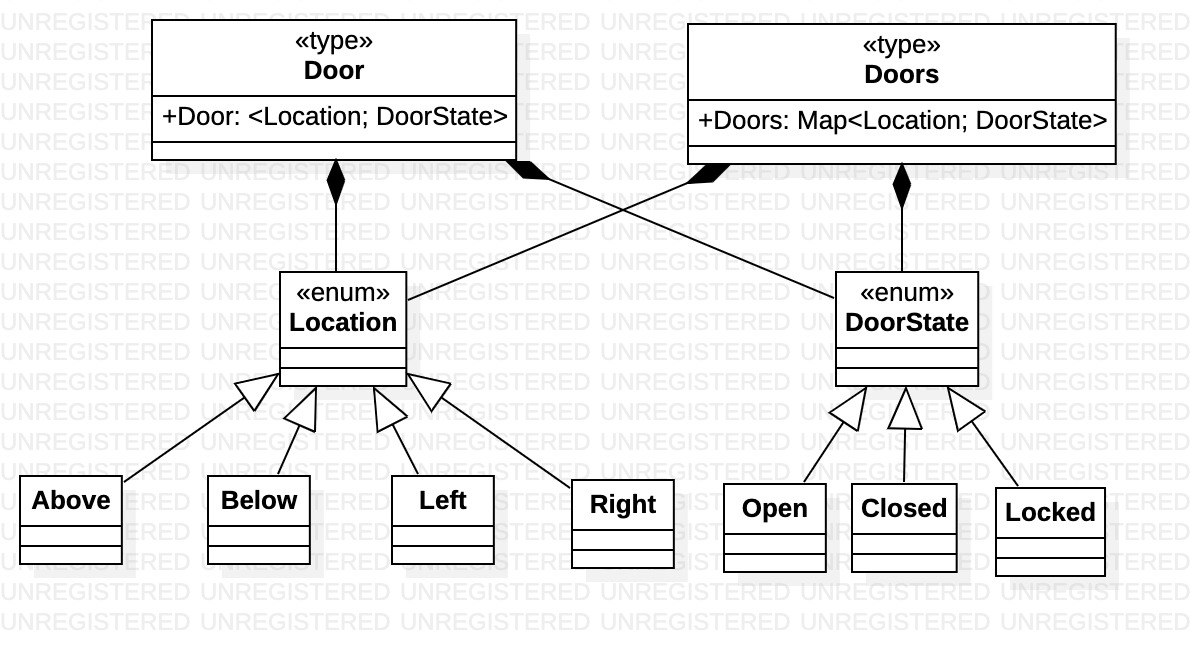
\includegraphics[scale=0.25]{DoorClassDiagram.jpg}
    \caption{\textit{Door class diagram(da modificare con versione pro di staruml)}} 
\end{figure}

\subsection{AnythingModel}
In generale ogni oggetto in gioco contiene un identificativo univoco e una bounding box che ne determina posizione e dimensioni 2D, inoltre ad ogni istanza è associata la factory per la sua View in modo tale che, quando una collezione di AnythingModel viene renderizzata, è sufficiente creare la View e chiamare il metodo draw. 

Ogni oggetto inoltre reagisce alla richiesta di update che avviene ad ogni iterazione del game loop, ma il modo con cui lo fa dipende da specifici comportamenti definiti come sottotipi mixabili di AnythingModel.

I sottotipi principali sono:
\begin{itemize}
    \item \textbf{DynamicModel} un oggetto in grado di spostarsi autonomamente durante un update, dove e come viene stabilito dalla classe che esegue il mixing attraverso l'implementazione di alcuni template-method predisposti
    \item \textbf{AliveModel} un oggetto vivo che può essere colpito perdendo vita. Non ha comportamento autonomo.
    \item \textbf{DamageModel} un oggetto che provoca danno di contatto. Non ha comportamento autonomo.
    \item \textbf{FireModel} un oggetto in grado di sparare autonomamente durante un update, dove e come viene stabilito dalla classe che esegue il mixing attraverso l'implementazione di alcuni template-method predisposti. Durante l'update può emettere uno ShotEvent contenente ShotModel
    \item \textbf{SolidModel} un oggetto solido che non può essere fisicamente attraversato da un altro. Non ha comportamento autonomo.
\end{itemize}

Questi tratti possono richiedere delle Stats per ottenere dei parametri al loro funzionamento (ad esempio la velocità massima da applicare ad uno spostamento): le Stats se richieste sono assegnate durante l'istanzazione di un Model ma possono cambiare durante il gioco.

Di seguito in figura 10 mostriamo un estratto della gerarchia di AnythingModel con tutti i sottotipi che aggiungono proprietà e comportamenti al Model di base e che possono essere estesi o mixati da un Model finale.

\begin{figure}[!hbt]
    \centering
    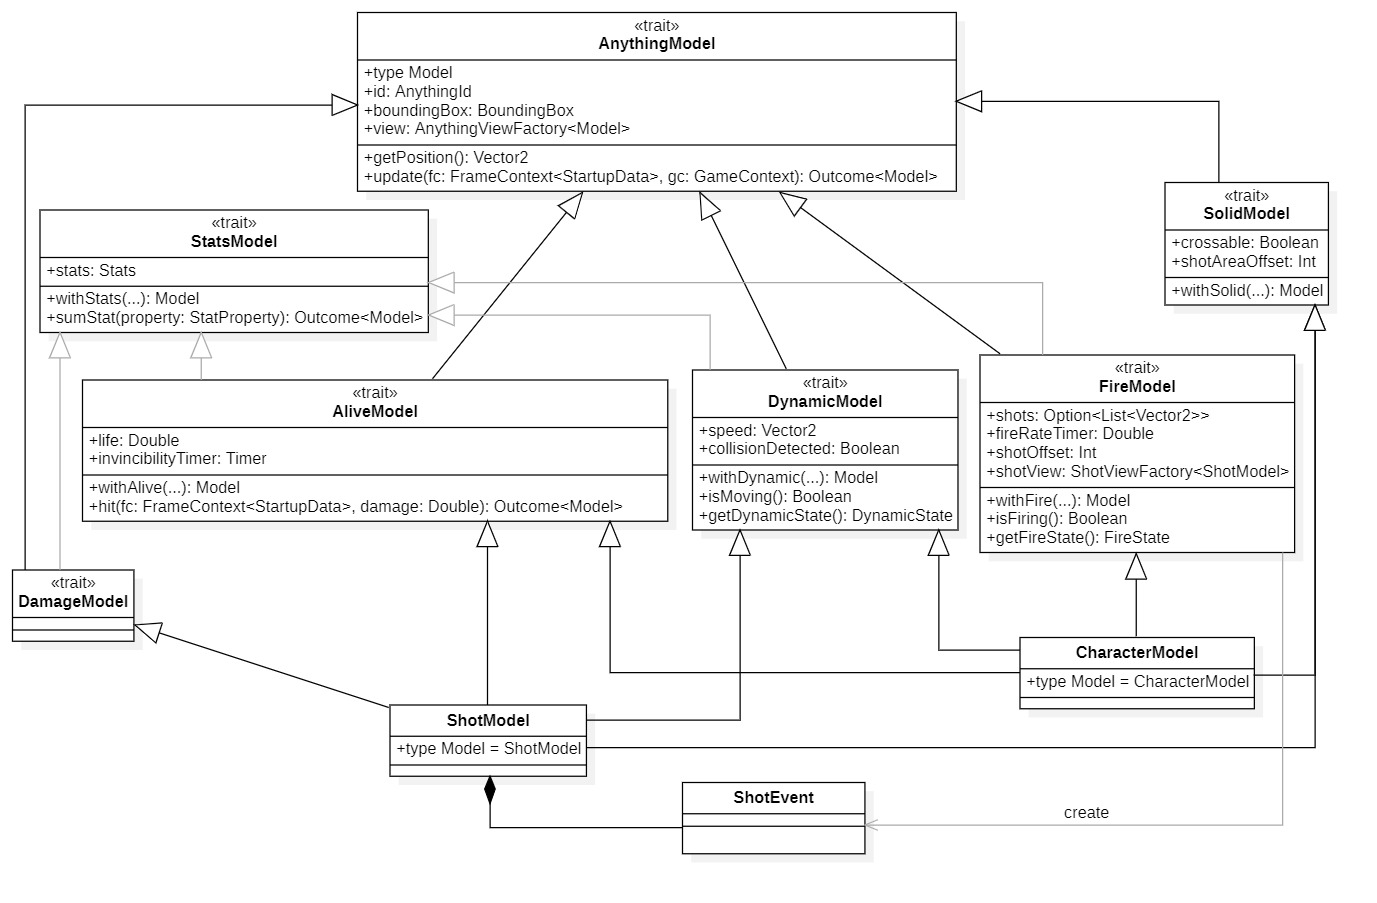
\includegraphics[scale=0.37]{AnythingModel.jpg}
    \caption{\textit{Gerarchia AnythingModel}} 
\end{figure}

\subsubsection{Update e immutabilità}

Ogni metodo che applica modifica al Model, a partire da update che viene richiamata ad ogni iterazione del game loop, deve ritornare una \textbf{copia aggiornata} dello stesso e del \textbf{tipo corrente}: adottiamo il pattern \textbf{F-Bounded Polymorphism con type-member}. 
Allo scopo predisponiamo un type member astratto Model e per ogni trait un template method with***(...) che accetta come argomenti quelli da modificare e ritorna un nuovo oggetto aggiornato di tipo Model: entrambi da definire nella classe finale che mixa il trait.
E' richiesto che il metodo update richiami super.update in modo da propagare l'aggiornamento a tutti i trait mixati.
\textit{Si rimanda all'implementazione per il dettaglio di come il pattern viene applicato con Scala.}

Per concludere, il metodo update riceve in input, oltre al FrameContext di Indigo, il \textbf{GameContext} che contiene lo stato della stanza corrente e il CharacterModel in modo da permettere all'oggetto in gioco comportamenti che si adattano alla situazione.

\paragraph{Nota} Sebbene una soluzione consigliata in sostituzione al polimorfismo F-Bounded è quella di impiegare polimorfismo ad-hoc con typeclass, abbiamo riscontrato che nel nostro caso volendo mantenere il mixing degli oggetti questo pattern non è facilmente applicabile e avrebbe generato più boilerplate code.

\paragraph{Nota}
Abbiamo deciso di inglobare il comportamento nei Model con il metodo update, ma un alternativa forse migliore e più semplice era delegarlo a sistemi esterni, i quali si sarebbero occupati ad esempio di spostare gli oggetti, farli sparare, etc: in questo progetto abbiamo cercato di emulare un modello ad agenti oltre che garantirci la massima possibilità di personalizzazione del comportamento soprattutto per quanto riguarda i nemici. 

\subsubsection{Gestione degli spari}
Riguardo a FireModel e agli spari \textbf{ShotModel} occorre specificare che:
\begin{itemize}
    \item possono essere sparati più colpi ShotModel contemporaneamente in direzioni diverse
    \item tra un colpo e l'altro deve trascorrere del tempo in base alla Stats "rate di fuoco"
    \item occorre generare il colpo a certo un offset rispetto alla posizione del oggetto che sta separando
    \item occorre specificare una ShotView factory da passare allo ShotModel, infatti in questo caso sono disponibili più View da utilizzare
\end{itemize}
FireModel durante un update genera l'evento \textbf{ShotEvent} indicando le proprietà dello ShotModel da istanziare (tra cui velocità e danno) ed inserendolo nella monade Outcome di ritorno: verrà gestito nell'iterazione successiva del game loop e aggiunto al RoomModel.

\subsubsection{Mini framework per i nemici}

Abbiamo pensato ad un mini framework che consenta la creazione rapida di nuovi nemici in modo da soddisfare i requisiti di possibili future espansioni.
Al centro abbiamo \textbf{EnemyModel}, il quale dispone di una coda di stati temporizzati che vengono processati uno dopo l'altro: questo permette la realizzazione di nemici che eseguono una sequenza di azioni.
Sono stati definiti dei comportamenti mixabili elementari come:
\begin{itemize}
    \item \textbf{Follower}: un nemico che insegue il character
    \item \textbf{FiresContinuosly}: un nemico che spara in continuazione nella direzione del character
    \item \textbf{KeepsAway}: un nemico che si mantiene a distanza dal giocatore
    \item \textbf{Traveller}: un nemico che segue un percorso indicato da una sequenza di punti
\end{itemize}

Abbiamo pensato di esprimerli come strategie da ri-utilizzare, quindi come mixin puri mediante il meccanismo dei \textbf{Self-types} anzichè renderli degli EnemyModel ereditando da questo: il concetto è che se si vuole sviluppare un nemico si estende direttamente EnemyModel e non uno di questi comportamenti "plugin".

Di seguito in figura 10 mostriamo come sono stati definiti i nemici a livello di Model, abbiamo evidenziato i 4 comportamenti base in azzurro e le classi finali che rappresentano i nemici implementati in giallo.

\begin{figure}[!hbt]
    \centering
    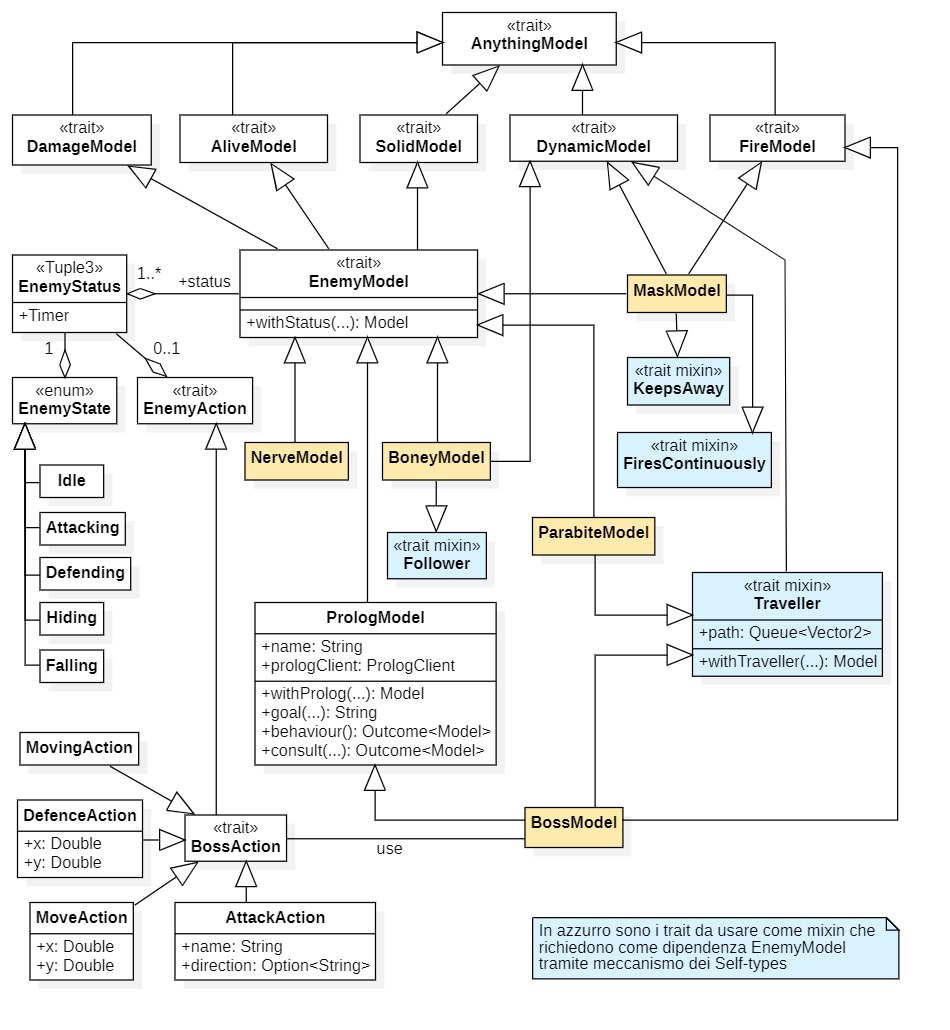
\includegraphics[scale=0.5]{Enemies.jpg}
    \caption{\textit{Gerarchia Enemies}}
\end{figure}

\subsection{AnythingView e AnythingViewModel}

Come scelta di design stabiliamo che 
\begin{itemize}
    \item Una View e un ViewModel devono essere progettati per uno specifico Model. 
    \item Un ViewModel potrebbe essere usato da diverse View
    \item Una View potrebbe non necessitare di un ViewModel: in generale quando non ha animazioni complesse
    \item Un ViewModel viene istanziato con lo stesso identificativo univoco usato per l'oggetto Model a cui si riferisce
    \item Un Model potrebbe disporre di diverse versioni di View ma la sua istanza ne utilizza una
\end{itemize}
Per la View abbiamo pensato di adottare il pattern \textbf{Family Polymorphism} definendo al suo interno i type member astratti \textbf{Model} e \textbf{ViewModel} che vengono concretizzati dai sottotipi della View.
Nella versione finale tuttavia i due tipi interni vengono collegati a dei parametri generici in quanto abbiamo trovato che questa soluzione
\begin{itemize}
    \item ci offre tutti i vantaggi di avere dei type member come la pulizia del codice o la possibilità di usare path-dependent types
    \item ci ha dato meno problemi di type inference 
    \item ci consente di risolvere il problema di type test runtime su tipi astratti \textit{(vedi approfondimento su implementazione)}
    \item a nostro avviso è più espressiva per indicare cosa richiede una View
\end{itemize}

Il pattern \textbf{Family Polymorphism} è stato applicato definendo il tipo astratto \textbf{View} che rappresenta il contenuto grafico da visualizzare attraverso il metodo \textbf{draw}, quest'ultimo richiama il template method \textbf{view} per ottenerlo.

\begin{figure}[!hbt]
    \centering
    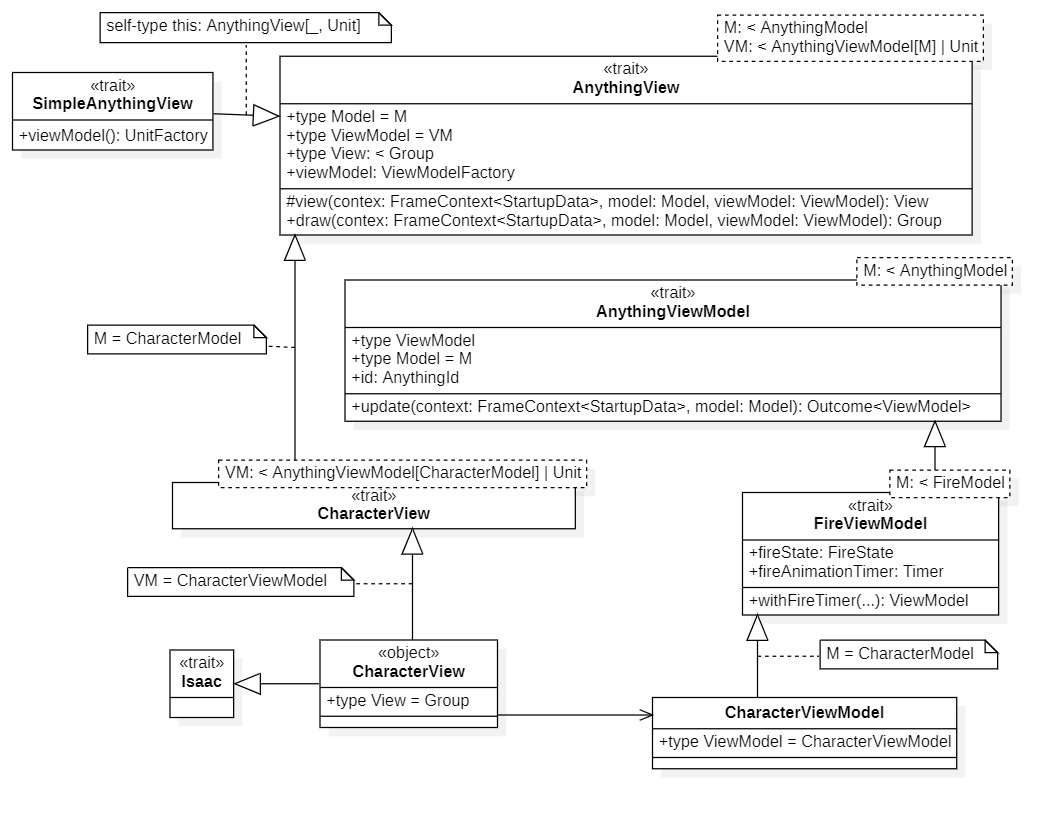
\includegraphics[scale=0.45]{AnythingViewModel.jpg}
    \caption{\textit{Gerarchia AnythingView e AnythingViewModel}} 
\end{figure}

In figura mostriamo l'utilizzo degli \textbf{Union Types} per definire che un ViewModel può non essere richiesto da una View.
Per la gerarchia di ViewModel valgono gli stessi concetti già menzionati per il Model di immutabilità e polimorfismo F-Bounded.
L'esempio concreto di utilizzo in figura riguarda il Character, ma è definito almeno un singleton object View per ciascun Model.

\subsubsection{Asset e animazioni}

\subsection{Sistema di controllo delle collisioni}
Il sistema di controllo delle collisioni ha l'obbiettivo di verificare se due elementi all'interno di una stanza collidono. 
Se questo accade, è necessario aggiornare la posizione degli elementi per evitare che gli elementi si intersechino e gestire un side effect che potrebbe o meno esserci durante la collisione (danno). 

Il sistema agisce e controlla solamente gli Anything di tipo Solid all'interno della stanza correntemente visualizzata.
Essendo il GameModel un'istantanea immutabile, il controllo avviene ad ogni Frame e su una struttura dati statica. 

Il sistema è composto da una serie di funzioni racchiusi in un modulo e sfruttato dal GameModel stesso, il quale va a controllare gli Anything presenti nella Room corrente e ritorna un modello aggiornato, come si può vedere in figura 6.

Il controllo è eseguito in due momenti distinti: 
\begin{enumerate}
  \item In un primo momento viene verificata la collisione tra un elemento e tutti gli altri interni alla stanza. Per ogni collisione viene applicata una funzione all'elemento che corrisponde al side effect.
  \item In un secondo momento vengono ricontrollate le collisioni e spostati gli elementi di conseguenza. 
\end{enumerate}

Il doppio controllo è dovuto al fatto che non è possibile spostare subito un elemento, perchè si potrebbero perdere collisioni con altri elementi.
Questo aspetto, in termini di prestazioni, è largamente migliorabile, ma si rimanda a eventuali sviluppi futuri.


\subsection{Pattern di progettazione}
Di seguito si elencano brevemente i pattern di progettazione utilizzati. 
\subsubsection{Family polimorphism}
Il family polimorphism è stato utilizzato in più di un occasione, tra cui
\begin{itemize}
    \item Definizione di una struttura per il Dungeon, ancora da tipare, ma che già definisce i comportamenti principali di esso.
\end{itemize}
\subsubsection{Bounded F-polimorphism}
\subsubsection{Pimp my library}
Il pattern Pimp my library è stato ampiamente utilizzato, soprattuto per quanto riguarda l'estensione di librerie scritte da terze parti, come ad esempio l'engine Indigo. 
Avendo usato Scala 3 è stato utilizzato il meccanismo degli \textit{extension} method.

In particolare è stata estesa la struttura dati Group di Indigo (rappresentante un gruppo di elementi visualizzabili a schermo), aggiungendo metodi comuni per centrare e scalare gli oggetti in base allo schermo.

Si è sfruttato il pattern anche per modellare le Door come solo struttura dati, per poi modellare i vari comportamenti mediante metodi esterni. Per questa struttura, si è quindi diviso lo stato dal comportamento. 

...andare avanti

\subsubsection{Strategy}
Il pattern strategy è stato utilizzato all'interno della logica di update delle strutture dati. Avendo lavorato con strutture dati immutabili, è stato molto utile definire una funzione comune di aggiornamento che accettasse una strategia di aggiornamento piuttosto che il vero aggiornamento, per via delle logiche a volte innestate che ci si è trovati ad affrontare. 
Un altro momento in cui si è rivelato utile questo pattern è stato all'interno del sistema di gestione delle collisioni, in cui, alla scoperta di una collisione, l'update dell'elemento dipendeva appunto da una strategia variabile. 
\subsubsection{Adapter}
Conversion

\subsection{Organizzazione del codice}
Il codice è stato organizzato in packages. Questi seguono la suddivisione in scene dell'applicativo. Al loro interno, si può ritrovare una suddivisione in Model, View, ViewModel e Componenti.
Il package Core invece, contiene le parti basilari a cui il resto del sistema fa riferimento.

\begin{figure}[!hbt]
    \centering
    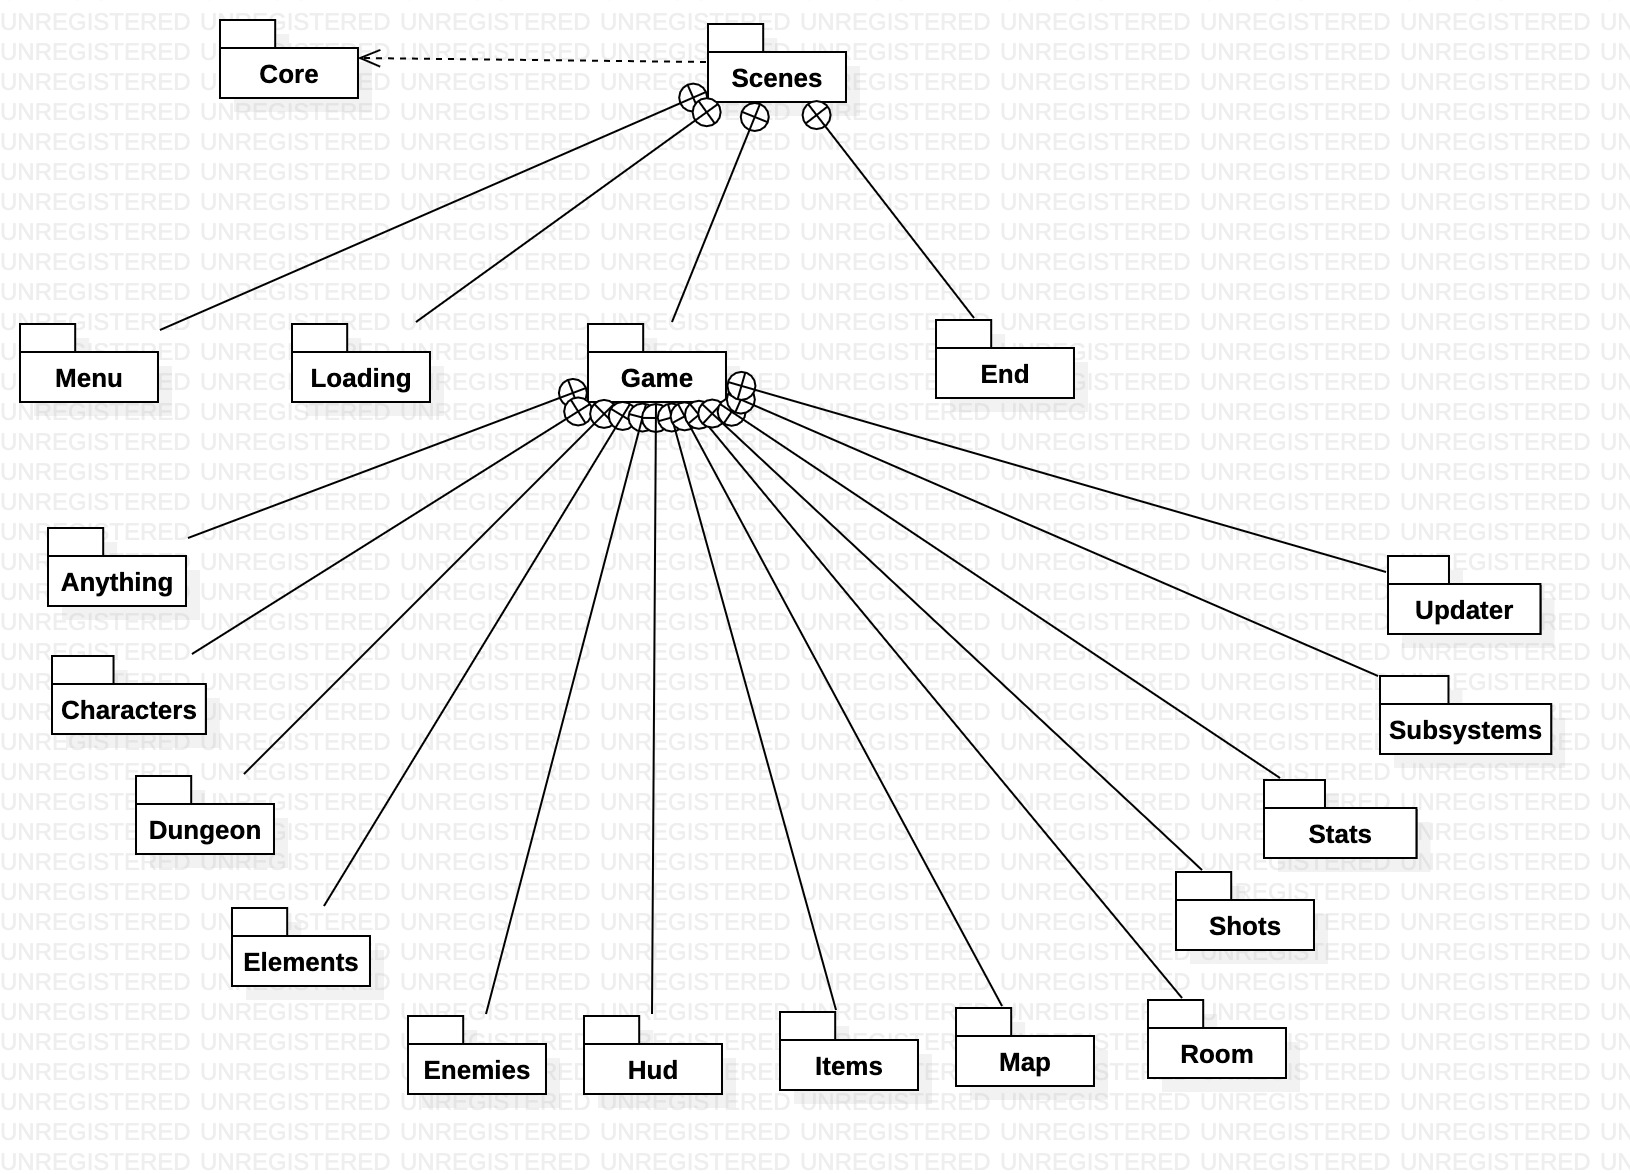
\includegraphics[scale=0.25]{package-diagram.jpg}
    \caption{\textit{Package Diagram del sistema(da modificare con versione pro di staruml)}} 
\end{figure}
\subsection{Alan Mancini}
Durante il corso del progetto mi sono occupato di studiare ed implementare:
\begin{itemize}
    \item AnythingModel con alcuni suoi sottotipi come DynamicModel e AliveModel e sperimentazione del workflow per consentire mixin/estensione e l'update del Model immutabile 
    \item Macro per ridurre il boilerplate code quando si estende un AnythingModel
    \item Adapter per semplificare l'update di un insieme di Anything
    \item AnythingView e AnythingViewModel di base e sperimentazione del workflow derivante
    \item Nemici per quanto concerne Model ed i loro comportamenti riutilizzabili
    \item PrologService come sottosistema di Indigo, integrazione di TauProlog e intefacciamento grazie a Scala.js, ed infine client per consultazioni da parte del gioco
    \item Generazione del dungeon randomica con Prolog
    \item Visualizzazione mini-mappa del dungeon
\end{itemize}
\subsubsection{AnythingModel e immutabilità}
Per quanto riguarda l'applicazione del pattern \textbf{F-Bounded Polymorphism} la soluzione che ho adottato con type-member anzichè l'utilizzo di argomenti generici garantisce un buon livello di type-safety: sembra difficile se non impossibile rompere i vincoli di tipo imposti.  
Impongo che il tipo di \textit{this} sia sottotipo di Model e quest'ultimo sottotipo del tratto in cui è definito: tutto questo permette anche di implementare un metodo update di base che ritorni proprio \textit{this} di tipo Model.

\begin{lstlisting}[language=Scala]
trait AnythingModel {
    type Model >: this.type <: AnythingModel
    
    val id: AnythingId
    val view: () => AnythingView[Model, _]

    ...

    def update(context: FrameContext[StartupData])(gameContext: GameContext): Outcome[Model] =
        Outcome(this)
    }
}  

trait DynamicModel extends AnythingModel with StatsModel {
  type Model >: this.type <: DynamicModel

  val speed: Vector2
  val collisionDetected: Boolean

  def withDynamic(boundingBox: BoundingBox, speed: Vector2, collisionDetected: Boolean): Model

  ...

  override def update(context: FrameContext[StartupData])(gameContext: GameContext): Outcome[Model] =
    for {
      superObj <- super.update(context)(gameContext)
      (newSpeed, newPosition) = computeMove(context)(gameContext)
      boundLocation           = gameContext.room.boundPosition(newPosition)
      newObj = superObj
        .withDynamic(boundLocation, newSpeed, boundLocation.position != newPosition.position)
        .asInstanceOf[Model]
    } yield newObj

} 
\end{lstlisting}

Da notare la necessità di un cast a Model in quanto il compilatore Scala non riconosce che il type member di ritorno è lo stesso definito poco sopra: questo cast comunque è legittimo e sicuro. 

Per concludere AnythingModel: la factory per la view è richiesta come funzione in linea con il \textbf{pattern strategy} applicato in modo funzionale con Scala.

Cambiando argomento, ho applicato il pattern \textbf{Pimp My Library} al fine di estendere le funzionalità di Double in modo da ottenere un Timer, utilizzato poi in diversi Model 
\begin{lstlisting}[language=Scala]
type Timer = Double
extension (timer: Timer)
    def elapsed(time: Double): Timer = timer match {
        case 0                 => 0
        case x if x - time > 0 => x - time
        case _                 => 0
    }
\end{lstlisting}

Infine ho utilizzato il \textbf{pattern Adapter} per trasformare implicitamente Vector2 in Vertex, due modi di Indigo per gestire i vettori secondo me ridondanti e per questo abbiamo deciso di utilizzarne uno solo nei nostri Model
\begin{lstlisting}[language=Scala]
given Conversion[Vector2, Vertex] with
    def apply(v: Vector2): Vertex = Vertex(v.x, v.y)
\end{lstlisting}



\subsubsection{Macro per ridurre boilerplate code}
Quando si definisce il Model di un oggetto di gioco che mixa diversi comportamenti è necessario implementare altrettanti template method  del tipo with*Comportamento*(...) in modo da permettere la sua copia aggiornata. 

\begin{lstlisting}[language=Scala]
def withDynamic(x,y,z) = copy(x=x,y=y,z=z); 
\end{lstlisting}

Per questo ho cercato un modo per generare in automatico questi metodi per una case class qualsiasi e l'unico sistema era scrivere una macro attivata da una annotation, ma Scala 3 al momento non supporta questa soluzione possibile su Scala 2.

Quindi ho implementato la \textbf{copyMacro} che consente di eseguire il metodo copy con come argomenti quelli dello scope dove viene attivata la macro, sfruttando le potenzialita della ancora non documentata Scala Reflection API. 

\begin{lstlisting}[language=Scala]
def withDynamic(x,y,z) = copyMacro
\end{lstlisting}

\subsubsection{Adapter per update di collection di Anything}

Quando si esegue l'update di una collezione di oggetti AnythingModel o AnythingViewModel ad esempio Map[AnythingId, AnythingModel] si ottiene una Map[AnythingId, Outcome[AnythingModel]] ma quello che occorre è ottenere la Map originale unendo le Outcome e gli eventi contenuti da ciascuna.

\begin{lstlisting}[language=Scala]
anythings.map((id, any) => id -> any.update(context)(GameContext(this, character)))
\end{lstlisting}

Per comodità ho applicato il \textbf{pattern Adapter} fornendo un apposito convertitore implicito, di seguito quello per AnythingViewModel.

\begin{lstlisting}[language=Scala]
given Conversion[Map[AnythingId, Outcome[AnythingViewModel[_]]], Outcome[Map[AnythingId, AnythingViewModel[_]]]] with
  def apply(set: Map[AnythingId, Outcome[AnythingViewModel[_]]]): Outcome[Map[AnythingId, AnythingViewModel[_]]] =
    set.foldLeft(Outcome(Map[AnythingId, AnythingViewModel[_]]().empty))((acc, el) =>
      acc.merge[AnythingViewModel[_], Map[AnythingId, AnythingViewModel[_]]](el._2)((set, el2) => set + (el._1 -> el2))
    )
\end{lstlisting}

\subsubsection{AnythingView e AnythingViewModel}

Nel codice che segue da notare è il context bound \textbf{Typeable} (alias di TypeTest[Any,T]) che importa ed abilita gli impliciti TypeTest[Any,M] e TypeTest[Any,VM] i quali ci permettono in modo molto veloce, pulito e sicuro di eseguire una draw dato un Model o ViewModel non correttamente tipati.


\begin{lstlisting}[language=Scala]
trait AnythingView[M <: AnythingModel: Typeable, VM <: AnythingViewModel[M] | Unit: Typeable] {
  type Model     = M
  type ViewModel = VM
  type View <: Group

  def viewModel: (id: AnythingId) => ViewModel

  protected def view(contex: FrameContext[StartupData], model: Model, viewModel: ViewModel): View
  
  ...

  def draw(contex: FrameContext[StartupData], model: Model, viewModel: ViewModel): Group =
    view(contex, model, viewModel)
        .moveTo(model.getPosition())
        .moveBy(Assets.Rooms.wallSize, Assets.Rooms.wallSize)
        .withDepth(depth(model))

  @targetName("anyDraw")
  def draw(contex: FrameContext[StartupData], model: AnythingModel, viewModel: AnythingViewModel[_] | Unit): Group =
    (model, viewModel) match {
      case (m: Model, vm: ViewModel) => draw(contex, m, vm)
      case _                         => Group()
    }
}
\end{lstlisting}

Il problema che avevamo nella visualizzazione degli Anything era che, data una loro collezione, non è possibile ottenere un suo singolo elemento tipato correttamente in modo automatico, quindi l'unica soluzione trovata prevedeva di fare pericolosi type cast.
Nel codice sotto ad esempio il Model genera la View sulla quale viene eseguita una draw: il Model passato alla draw non veniva riconosciuto dal compilatore del tipo richiesto e soprattutto il ViewModel cercato nell'altra collezione viene ovviamente tipato in modo generico. 
Ho quindi pensato di invertire il problema permettendo al metodo draw della View di accettare un qualsiasi Model o ViewModel in modo sicuro eseguendo un \textbf{type check del tipo a runtime} verificando che questo corrisponda ai type member specificati.
Il TypeTest interviene implicitamente durante il match con i type Member della View.

\begin{lstlisting}[language=Scala]
def anythingView(context: FrameContext[StartupData], model: RoomModel, viewModel: RoomViewModel): Group =
    model.anythings.foldLeft(Group())((s1, s2) =>
      s1.addChild(
        s2._2
          .view()
          .draw(
            context,
            s2._2,
            viewModel.anythings
              .get(s2._2.id)
              .getOrElse[AnythingViewModel[_] | Unit](())
          )
      )
    )
\end{lstlisting}   

L'utilizzo di \textbf{Typeable} è presente anche in \textbf{AnythingViewModel} dove il suo metodo update richiede in input un oggetto di tipo Model generalmente ottenuto da una collezione mista.

\subsubsection{Nemici e comportamenti come mixin puri}

Per quanto riguarda il mini framework per lo sviluppo di nemici ho applicato il pattern \textbf{Pimp My Library} al fine di creare un \textbf{mini DSL} per generare la coda di stati a partire da due di essi 

\begin{lstlisting}[language=Scala]
extension (s1: EnemyStatus) def :+(s2: EnemyStatus): Queue[EnemyStatus] = Queue(s1, s2)
\end{lstlisting} 

Circa i comportomenti dei nemici, mostro qui un esempio dell'impiego dei \textbf{Self-types} per evitare di estendere da EnemyModel
\begin{lstlisting}[language=Scala]
trait Follower { this: EnemyModel with DynamicModel =>
  def computeSpeed(context: FrameContext[StartupData])(gameContext: GameContext): Vector2 =
    status.head match {
      case (EnemyState.Attacking, _) =>
        (gameContext.character.getPosition() - getPosition()).normalise * MaxSpeed @@ stats
      case _ => Vector2.zero
    }
}
\end{lstlisting} 

\subsubsection{PrologService}
Riguardo l'implementazione dei Term prolog ho proceduto secondo la modalita \textbf{Mixed OOP/FP} separando la definizione dei dati dal comportamento. Si è poi reso utile l'impiego del pattern \textbf{Adapter} per convertire implicitamente all'occorrenza i termini Tau in nostri Term.
\begin{lstlisting}[language=Scala]
given Conversion[TauTerm, Term] with
  def apply(t: TauTerm): Term = t.args.length match {
    case 0 => Atom(t.id)
    case _ =>
      Struct(
        Atom(t.id),
        t.args
          .map[Term](arg =>
            arg match {
              case a: TauNum  => a
              case a: TauVar  => a
              case a: TauTerm => a
            }
          )
          .toList: _*
      )
  }

given Conversion[TauSubstitution, Substitution] with
  def apply(t: TauSubstitution): Substitution = Substitution(
    t.links.foldLeft(HashMap[String, Term]())((hmap, kv) => hmap + (kv._1 -> kv._2))
  )
\end{lstlisting} 

\subsubsection{Generazione dungeon con Prolog}
L'algoritmo Prolog genera il dungeon partendo dalla stanza iniziale posizionata in 0,0 all'interno di una griglia virtualmente infinita. 
Le successive stanze vengono posizionate selezionando randomicamente una cella libera adiacente a quelle già aggiunte. 
Per fare questo viene mantenuta una lista di posizioni libere, questa inoltre viene troncata sempre per mantenere una lunghezza di 6 posti in modo che l'algoritmo proceda ad aggiungere stanze con buona probabilità partendo dall'ultima stanza generando così una struttura più "tortuosa" come da requisito.
La stanza del boss, aggiunta per ultima, viene posizionata in modo da essere adiacente ad una sola stanza.
\subsection{Federico Mazzini}
Durante il corso del progetto mi sono occupato di differenti parti all'interno di esso, tra cui, in ordine:
\begin{itemize}
    \item Scena di loading e caricamento degli asset
    \item Il Dungeon, dal modello alla sua integrazione con le altre componenti (ad eccezione dell'algoritmo Prolog per la sua generazione)
    \item Le stanze di gioco, la loro tipologia, i diversi comportamenti e la gestione degli Anything interni
    \item Le porte e il passaggio da una stanza all'altra
    \item Definizione e visualizzazione di elementi bloccanti
    \item Disposizione, mediante Prolog, di nemici ed elementi bloccanti all'interno delle stanze
    \item Sistema delle collisioni e di Bounding degli elementi interni alla stanza
    \item Scena finale e relativa verifica di avvenuta vittoria/sconfitta
\end{itemize}

\subsubsection{Dungeon}
Per quanto riguarda il Dungeon, ho cercato di fornire un'implementazione basilare del modello e delle sue funzioni principali. 
In particolare ho immaginato la mappa come una griglia, composta da una collezione di elementi in posizioni [X,Y]. Questi elementi sarebbero poi diventate le stanze all'interno del Dungeon effettivo, 
ma per la generazione, è stato utile ridurli a semplici "tipi", da definire successivamente, perciò ho messo in pratica il pattern \textbf{Family Polimorphism}.

\begin{lstlisting}
type Position = (Int, Int)
trait Grid {
    type Room
    val content: Map[Position, Room]
    val initialRoom: Position
  }   
\end{lstlisting}
Il type Room è stato ridefinito in due case class, la prima è stata utilizzata durante la generazione del dungeon, prima di generare gli elementi interni alla stanza. 
In questo caso Room è stato associato ad un semplice enum descrivente il tipo di room. 

La seconda volta invece, è stato definito per il vero Dungeon, già generato e con elementi all'interno, in cui il type Room è stato effettivamente associato al vero e completo modello della stanza.

\subsubsection{Room}
Come già descritto, le stanze sono di diverso tipo, Empty, Arena, Item e Boss. Per modellare questi concetti ho definito un trait base il quale contiene la maggior parte dei comportamenti ma lascia il resto alle classi specializzate. 
Una room, qualsiasi, è caratterizzata da un insieme di porte (link ad altre room), una collezione di Anything e un area di gioco in cui gli elementi si muovono. 
Avendo lavorato con strutture dati immutabili, ho cercato di fornire più metodi possibili per la modifica di una Room, intesa come creazione di un nuovo modello con la modifica specificata. Per evitare ripetizioni di codice, la funzione generale sfrutta le \textbf{Higher Order Function} e mette in campo il pattern \textbf{strategy}. 
\begin{lstlisting}
    def updateAnythings
    (updateFunc: Map[AnythingId, AnythingModel] => 
    Outcome[Map[AnythingId, AnythingModel]]): Outcome[RoomModel] =
    for (ua <- updateFunc(anythings))
      yield this match {
        case room: EmptyRoom =>
          room.copy(anythings = ua)
        case room: ItemRoom =>
          room.copy(anythings = ua)
        case room: ArenaRoom =>
          room.copy(anythings = ua)
        case room: BossRoom =>
          room.copy(anythings = ua)
        case _ => this
      }
\end{lstlisting}

Ho sfruttato questa funzione in molte altre adibite alla modifica degli Anything interni di una room, come ad esempio 
\begin{lstlisting}
  def addShot(shot: ShotModel): Outcome[RoomModel] =
    updateAnythings(anythings => 
        Outcome(anythings + (shot.id -> shot)))
\end{lstlisting}

\subsubsection{Door}
Per quanto riguarda le porte, ho cercato di rimanere il più fedele possibile allo stile funzionale. Ho perciò definito un tipo Location e un tipo State, i quali insieme vanno a comporre una porta.
Ho creato un object per permettermi di definire e modificare una Door, ma ciò che nella pratica ho utilizzato sono le \textbf{Extension} e le \textbf{Conversion} di scala 3 (impliciti precedentemente).
In questo modo, è possibile definire una collezione di porte per una stanza nel seguente modo: 
\begin{lstlisting}
    (Left -> Open) :+ (Right -> Open) :+ (Above -> Lock)
\end{lstlisting}

\subsubsection{Prolog}
Ho utilizzato il prolog per la definizione di un "area di gioco" e un "area elementi" all'interno delle stanze. Ho immaginato come il pavimento di una stanza fosse una griglia. 
Ho generato, aiutandomi con una findall, la griglia e, in base alle porte della stanza, un'area di gioco di dimensione variabile che comprendesse le porte. 
Ciò che non rientrava nell'area di gioco è stato classificato come area elementi.
Utilizzare il Prolog in questa situazione è stato molto utile per la natura "esplorativa" di esso, la quale mi ha permesso di calcolare facilmente le aree. Di contro, l'algoritmo da me sviluppato è relativamente lento considerando il resto del sistema. 

\subsubsection{Monadi}
All'interno del progetto è stata utilizzata la struttura monadica Outcome propria di Indigo. 
Attraverso essa è stato possibile wrappare l'intero modello o sottoparti di esso, concatenando diverse modifiche al modello senza avere side effect. Per lavorare con questa monade, ho utilizzato spesso la \textbf{for comprehension} di Scala. 
Di seguito un esempio, riguardante l'intera catena di update del modello di gioco. 
\begin{lstlisting}
    for {
            updatedCharacter <- model.updateCharacter(c => character.update(context)(gameContext))
            updatedRoom      <- updatedCharacter.updateCurrentRoom(r => model.currentRoom.update(context)(character))
            withPassage      <- updatedRoom.updateWithPassage
            withStats        <- withPassage.updateStatsAfterCollision(context)
            withMovements    <- withStats.updateMovementAfterCollision
          } yield withMovements
\end{lstlisting}
\subsection{Matteo Brocca}
Durante il corso del progetto mi sono occupato di studiare ed implementare:
\begin{itemize}
	\item Rappresentazione grafica degli Anythings tramite Asset ed animazioni
    \item Definizione del FireModel e ShotModel per la gestione dei proiettili
    \item Gestione delle statistiche degli Anythings
    \item Character controllato dal giocatore
    \item Boss, PrologEnemyModel e definizione del suo comportamento tramite Prolog
    \item Item che il Character può raccogliere per modificare le proprie statistiche
    \item HUD per la visualizzazione delle statistiche a schermo
\end{itemize}

\subsubsection{Rappresentazione grafica degli Anythings tramite Asset ed animazioni}
È stata creata una libreria per gli \textbf{AnythingAsset}, 
la quale codifica le informazioni di base necessare a disegnare a schermo un certo Asset ed implementa metodi condivisi. 

Questa organizzazione ci ha permesso di generare velocemente le specifiche View per Character, Enemies, Bosses, Items and Elements.

Facciamo un esempio:
Il CharacterModel, viene rappresentato a schermo dalla sua relativa CharacterView e CharacterViewModel 
che estendono relativamente da AnythingView ed AnythingViewModel

La CharacterView definisce solo la funzione di "disegno" che sfrutta il metodo drawComponents di AnythingAsset 
e viene mixata con il tipo di carattere che si vuole disegnare a schermo, in questo caso Isaac.
Il trait Isaac estende IsaacAsset per definire come disegnare ogni singolo componente a schermo.
A sua volta il trait IsaacAsset è quello che estende il trait base AnythingAsset 
e definisce le dimensioni e nome della Sprite che viene caricata durante l'avvio del gioco.

Nel momento in cui si decida di modificare l'estetica del Character (il \textit{"cosa"}), da "Isaac" a "Mario",
senza dover modificare il \textit{"come"} questo viene rappresentato (da una testa, un corpo, un ombra, ...),
basterà create un nuovo trait Mario e relativo MarioAsset.

\begin{lstlisting}[language=Scala]
trait AnythingAsset {
	...
	protected def drawComponents(components: List[SceneNode]): Group = ...
}

trait IsaacAsset extends AnythingAsset {
  	...
}

trait Isaac extends IsaacAsset{
	...
	def headView(model: CharacterModel, viewModel: CharacterViewModel): Graphic[Material.Bitmap] = {...}
	def bodyView(model: CharacterModel): Sprite[Material.Bitmap] = = {...}
}

trait CharacterView[VM <: AnythingViewModel[CharacterModel] | Unit] extends AnythingView[CharacterModel, VM] {}

object CharacterView extends CharacterView[CharacterViewModel] with Isaac {
	...
	def view(contex: FrameContext[StartupData], model: Model, viewModel: ViewModel): View =
		...
		drawComponents(List(shadowView, bodyView(model), headView(model, viewModel)))
}
\end{lstlisting}	

\subsubsection{Definizione del FireModel e ShotModel per la gestione dei proiettili}
Ogni proiettile generato dal FireModel è uno ShotModel.

La factory che ne permette la creazione durante la generazione dell'evento ShotEvent 
richiede anche quale sia la relativa View per la rappresentazione grafica del proiettile.
Si può infatti notare che il FireModel richiede la definizione della funzione di creazione di questa View di tipo ShotView (pattern strategy: factory as a function), un trait che sfrutta il \textbf{Self-Type} per richiedere espressamente di essere mixato 
con il trait \textbf{ShotAsset} che definisce le informazioni di base che ogni proiettile deve avere ed implementa la funzione \textbf{drawShot}

\begin{lstlisting}[language=Scala]
trait FireModel extends AnythingModel with StatsModel {
  	type Model >: this.type <: FireModel

	...

  	val shotView: () => ShotView[_]

  	...
}

class SingleShotView extends ShotView[Unit] with SimpleAnythingView {
  this: ShotAsset =>
  type View = Group

  def view(contex: FrameContext[StartupData], model: Model, viewModel: ViewModel): View =
    drawComponents(List(drawShot))

  ...
}
\end{lstlisting}

Un esempio dell'utilizzo del FireModel si può apprezzare all'interno del CharacterModel 
dove viene definita la shotView come un SingleShotView con il trait ShotBlue
e viene implementato il computeFire con il mapping dei tasti premuti dall'utente.

\begin{lstlisting}[language=Scala]
case class CharacterModel(...) extends AliveModel
		with DynamicModel
		with FireModel
		with DamageModel
		with SolidModel {

	val shotView        = () => new SingleShotView() with ShotBlue
	
	...
}
\end{lstlisting}

\subsubsection{Gestione delle statistiche degli Anything}
Si è realizzato il trait \textbf{StatsModel} da mixare con un qualsiasi Anything 
per gestire l'aggiornamento di queste caratteristiche nell'ambito dell'immutabilità.

Il metodo "sumStat" è l'unico utilizzato realmente all'interno del gioco e permette di 
aggiornare il valore di una determinata caratteristica sommando il valore proveniente da un Item raccolto 
verificando in automatico che il valore non diventi negativo.

Gli altri metodi "changeStats" e "changeStat" sono solo stati previsti per eventuali sviluppi futuri.  

\begin{lstlisting}[language=Scala]
trait StatsModel {
  type Model >: this.type <: StatsModel

  val stats: Stats

  def withStats(stats: Stats): Model

  def changeStats(context: FrameContext[StartupData], newStats: Stats): Outcome[Model] = Outcome(withStats(newStats))

  def changeStat(context: FrameContext[StartupData], property: StatProperty): Outcome[Model] =
    Outcome(withStats(stats + property))

  def sumStat(context: FrameContext[StartupData], property: StatProperty): Outcome[Model] =
    Outcome(withStats(stats +++ property))
}
\end{lstlisting}

Questo trait usufruisce della libreria \textbf{Stats} la quale è implementata seguendo il pattern \textbf{Pimp My Library} 
per mettere a disposizione i propri metodi all'interno dello specifico dominio applicativo (\textbf{DSL}).

La libreria definisce che cosa sono le Stats, una mappa di proprietà da nome a valore.
Sono stati implementate delle \textbf{Conversion} per utilizzare i valori definiti come Double anche in situazioni 
dove si accettano Int o String.
Inoltre sono state realizzate delle \textbf{extension} per definire operatori specifici per manipolarle.

\begin{lstlisting}[language=Scala]
package lns.scenes.game.stats

enum PropertyName:
	case 	MaxLife, Invincibility, MaxSpeed, Range, KeepAwayMin, KeepAwayMax, Damage, 
		FireDamage, FireRange, FireRate,FireSpeed

type PropertyValue = Double
type StatProperty  = (PropertyName, PropertyValue)
type Stats         = Map[PropertyName, PropertyValue]

given Conversion[PropertyValue, Int] with
	def apply(v: PropertyValue): Int = v.toInt

given Conversion[PropertyValue, String] with
	def apply(v: PropertyValue): String = v.toString

extension (p: PropertyValue) {
	def |+|(v: PropertyValue): PropertyValue = p match {
	case p if (v + p) < 0 => 0
	case _                => BigDecimal(v + p).setScale(2, BigDecimal.RoundingMode.HALF_UP).toDouble
	}
}

extension (p: PropertyName) {
	def @@(s: Stats): PropertyValue = s.getOrElse(p, 0.0)
}

extension (stats: Stats) {
	def +++(p: StatProperty): Stats =
	stats + stats.get(p._1).map(x => p._1 -> (x |+| p._2)).getOrElse(p)
}
\end{lstlisting}

\subsubsection{Boss, PrologEnemyModel e definizione del suo comportamento tramite Prolog}
Per la creazione del boss, il cui comportamento è definito tramite linguaggio Prolog, è stato creato il trait \textbf{PrologEnemyModel}. 
Grazie a Scala 3, il trait accetta il paramentro "\textit{name}" che definisce il nome del file prolog da interrogare e che sarà stato opportunamente caricato tra gli asset di gioco.

Se il suo EnemyStatus attuale (tipico degli EnemyModel) è di tipo \textit{Idle} e non è definita nessuna \textit{EnemyAction}, 
allora viene interrogato il codice Prolog. 
Il \textbf{goal} che viene passato è una stringa prodotta dal metodo del quale si richiede l'override.
La risposta del prolog, catturata dal gameLoop, esegue il metodo \textbf{behaviour} del chiamante implementato dalla classe che lo estende. 

\begin{lstlisting}[language=Scala]
trait PrologEnemyModel(name: String) extends EnemyModel {
  type Model >: this.type <: PrologModel

  val prologClient: PrologClient

  def withProlog(prologClient: PrologClient): Model

  protected def goal(context: FrameContext[StartupData])(gameContext: GameContext): String

  def behaviour(response: Substitution): Outcome[Model]

  protected def consult(context: FrameContext[StartupData])(gameContext: GameContext): Outcome[Model] = ...

  override def update(context: FrameContext[StartupData])(gameContext: GameContext): Outcome[Model] = ...
}

case class BossModel(...) ) 
	extends PrologEnemyModel("loki")
	with FireModel
	with Traveller {

	...

	protected def goal(context: FrameContext[StartupData])(gameContext: GameContext): String = ...

	def behaviour(response: Substitution): Outcome[Model] = ...
}
\end{lstlisting}

Il boss di nome "Loki" che è stato implementato può eseguire 5 diverse azioni, 3 di attacco, 1 di movimento ed 1 di difesa,
che hanno una probabilità in base allo stato di vita del Boss e del Character. 
Viene definito \textit{low} il livello di vita se questo è inferiore al 50\% della vita massima, altrimenti \textit{high}

\begin{lstlisting}[language=Scala]
% estratto del file prolog "assets/prolog/loki.pl"
... 
% List of probability value for actions based on Boss and Character life level
% @high|low (Boss)
% @high|low (Character)
% -Probability List[Attack, Defense, Move]
getActionsProbability(high, high, [0.7, 0.0, 1.0]).
getActionsProbability(high, low,  [0.5, 0.0, 1.0]).
getActionsProbability(low,  high, [0.7, 1.0, 0.0]).
getActionsProbability(low,  low,  [0.5, 0.7, 1.0]).
...
\end{lstlisting}

Di seguito vengono descritte nel dettaglio le singole azioni:
\begin{itemize}
	\item attack1(direction): viene generato un proiettile nella direzione del Character se questo si trova sullo stesso asse x o y.
	\item attack2: vengono generati 4 proiettili in contemporanea lungo i 2 assi x, y
	\item attack3: vengono generati 4 proiettili in contemporanea in diagonale lungo i 2 assi x, y
	\item move(x,y): il boss sposta rapidamente verso il punto x, y occupato dal Character
	\item defence(x,y): il boss si teletrasporta nel punto x,y se questo non è occupato da una roccia, altrimenti viene cercato il primo posto disponibile nel suo intorno
\end{itemize}
\section{Retrospettiva}
%Restrospettiva (descrizione finale dettagliata dell'andamento dello sviluppo, del backlog, delle iterazioni; commenti finali)
%Si noti che la retrospettiva è l'unica sezione che può citare aneddoti di cosa è successo in itinere, mentre le altre sezioni fotografino il risultato finale. Se gli studenti decideranno (come auspicato) di utilizzare un product backlog e/o dei backlog delle varie iterazioni/sprint, è opportuno che questi siano file testuali tenuti in versione in una cartella "process", così che sia ri-verificabile a posteriori la storia del progetto.

\subsection{Sprint 1 27/09 - 03/10}
\paragraph{Epic} Visualizzare il personaggio a schermo

Il primo sprint è stato prevalentemente organizzativo ed è stato focalizzato sulla scelta e il setup degli strumenti, la definizione del processo di sviluppo e il design architetturale. 
In particolare si è scelto di lavorare con il framework Indigo e si è studiata la sua documentazione, al fine di comprendere come organizzare il codice e poter definire l’architettura generale del gioco. 
Era previsto anche il setup della CI/CD, abbiamo deciso però di spostarla nella seconda sprint, la quale sarà orientata a implementare la struttura base e produrre la prima schermata di gioco. 


\begin{figure}[!hbt]
    \centering
    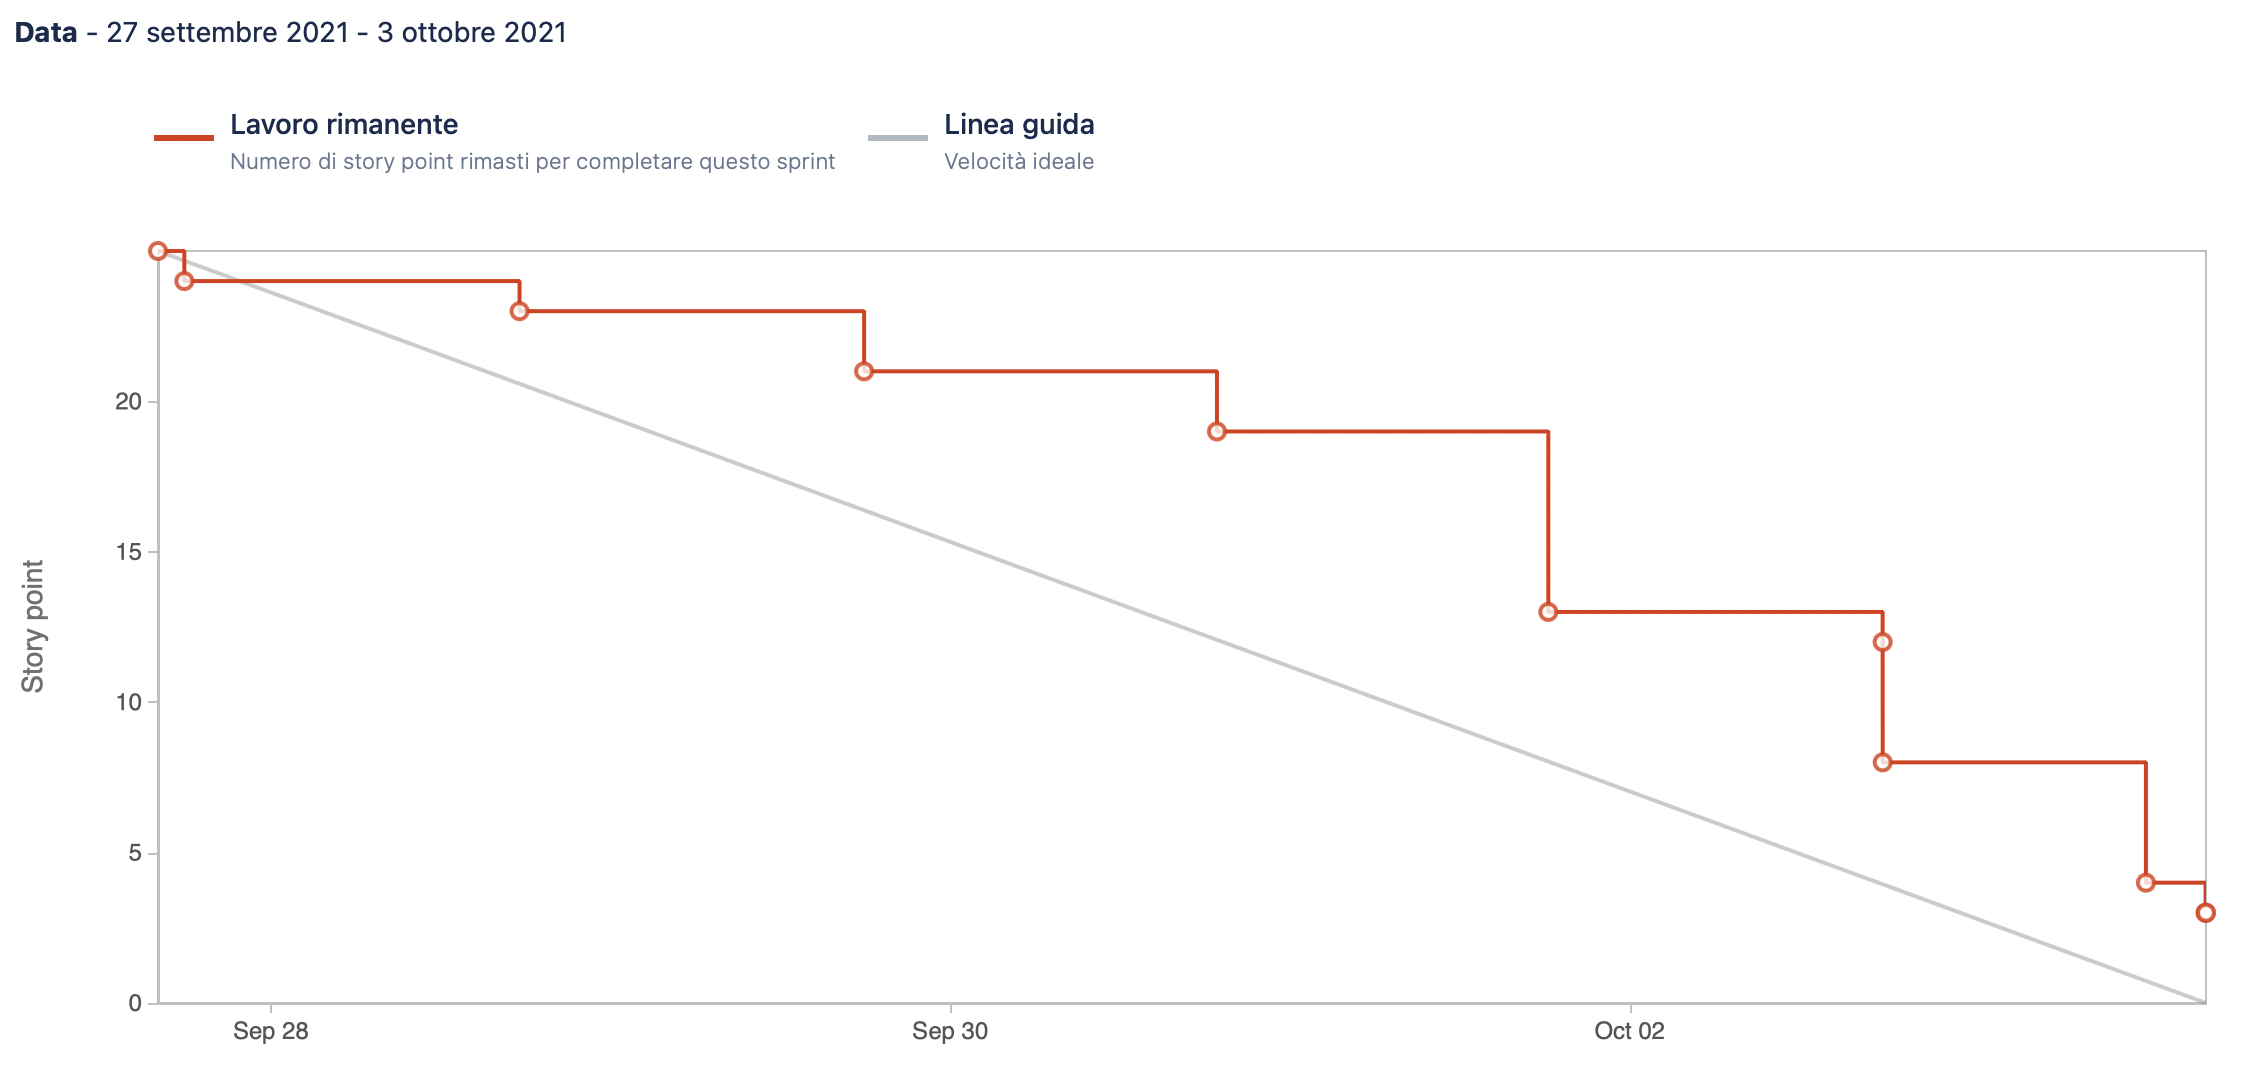
\includegraphics[scale=0.4]{sprint-1-burn-down.png}
    \caption{\textit{Grafico Burn-down primo sprint}} 
\end{figure}


\subsection{Sprint 2 04/10 - 10/10}
\paragraph{Epic} Visualizzare il personaggio a schermo

Nel secondo sprint abbiamo effettuato il setup dell'architettura includendo Indigo, al fine di visualizzare il menu di avvio, il loading e permettere all'utente di visualizzare il proprio personaggio all'interno di una stanza vuota. 
Abbiamo inoltre abilitato la continuous integration. Siamo così giunti all'obbiettivo dell'epic. In questa sprint, abbiamo fatto i primi passi con l'engine Indigo, confrontandoci costantemente in modo da sperimentare insieme il suo utilizzo. Questo ci ha permesso di allineare la nostra conoscenza a riguardo e definire una modalità operativa per le future sprint. 
Non siamo riusciti a completare la visualizzazione del personaggio in quanto ci siamo resi conto di dover impostare meglio il modello generale al fine di realizzare una struttura a componenti che funzioni con Indigo.

\begin{figure}[!hbt]
    \centering
    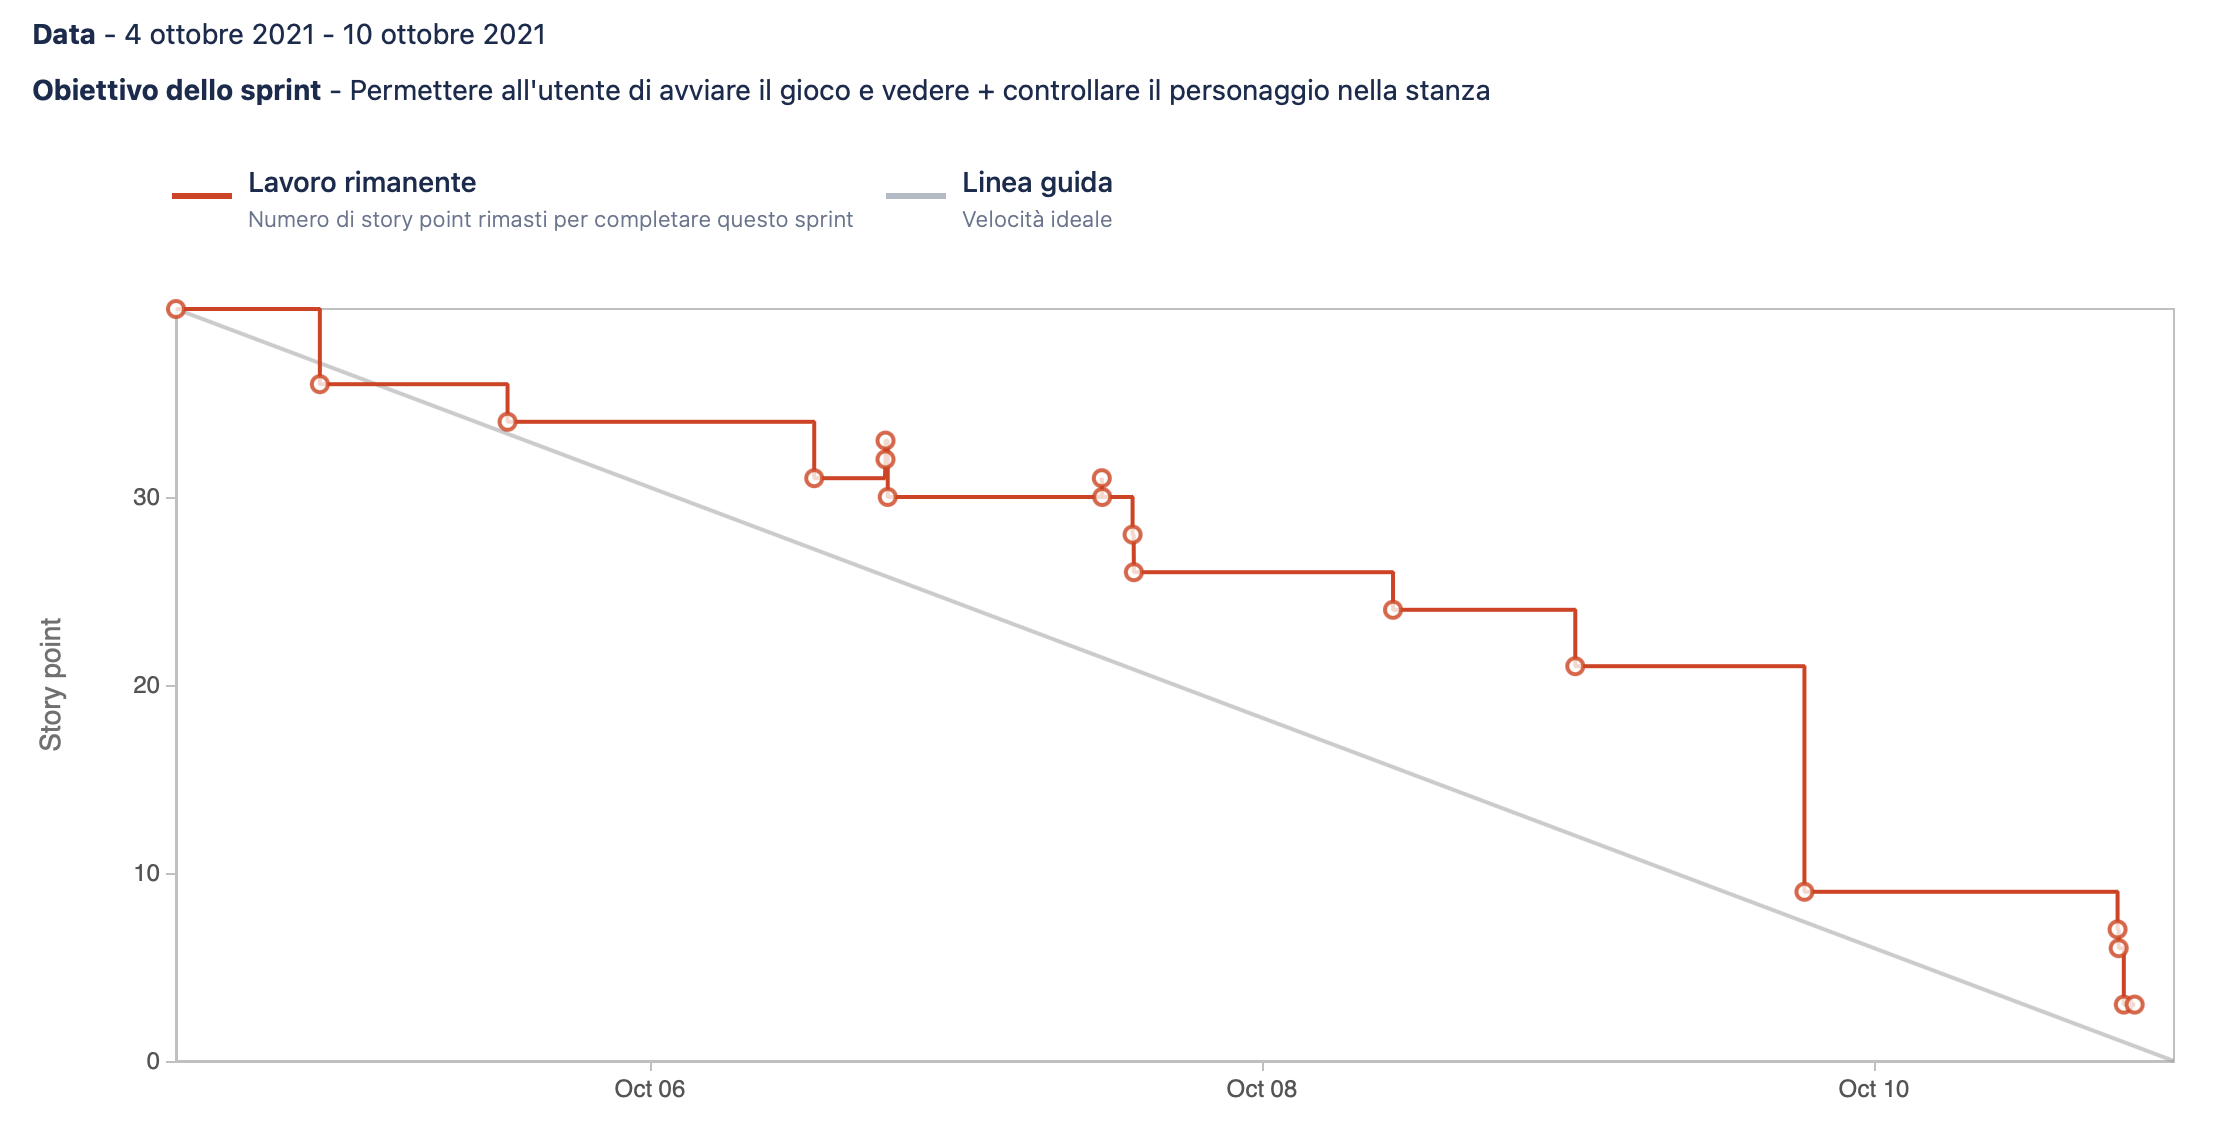
\includegraphics[scale=0.4]{sprint-2-burn-down.png}
    \caption{\textit{Grafico Burn-down primo sprint}} 
\end{figure}

\subsection{Sprint 3 11/10 - 17/10}

Il terzo sprint è stato dedicato al rifinimento del personaggio aggiungendo animazioni e vincolandolo all'interno dei confini della stanza. 
Questo ha richiesto di approfondire lo studio di Indigo riguardo le animazione e rifattorizzare la stanza, le sue proprietà e la sua logica. 
Oltre a questo è stata rivista la gerarchia di classi che supportano il personaggio e che sarà alla base di tutti gli elementi presenti dentro alla stanza (nemici, oggetti, elementi bloccanti).
Infine, con lo studio di un workflow di test per Indigo, ci siamo predisposti per uno sviluppo TDD che avverrà dalle prossime sprint.


\begin{figure}[!hbt]
    \centering
    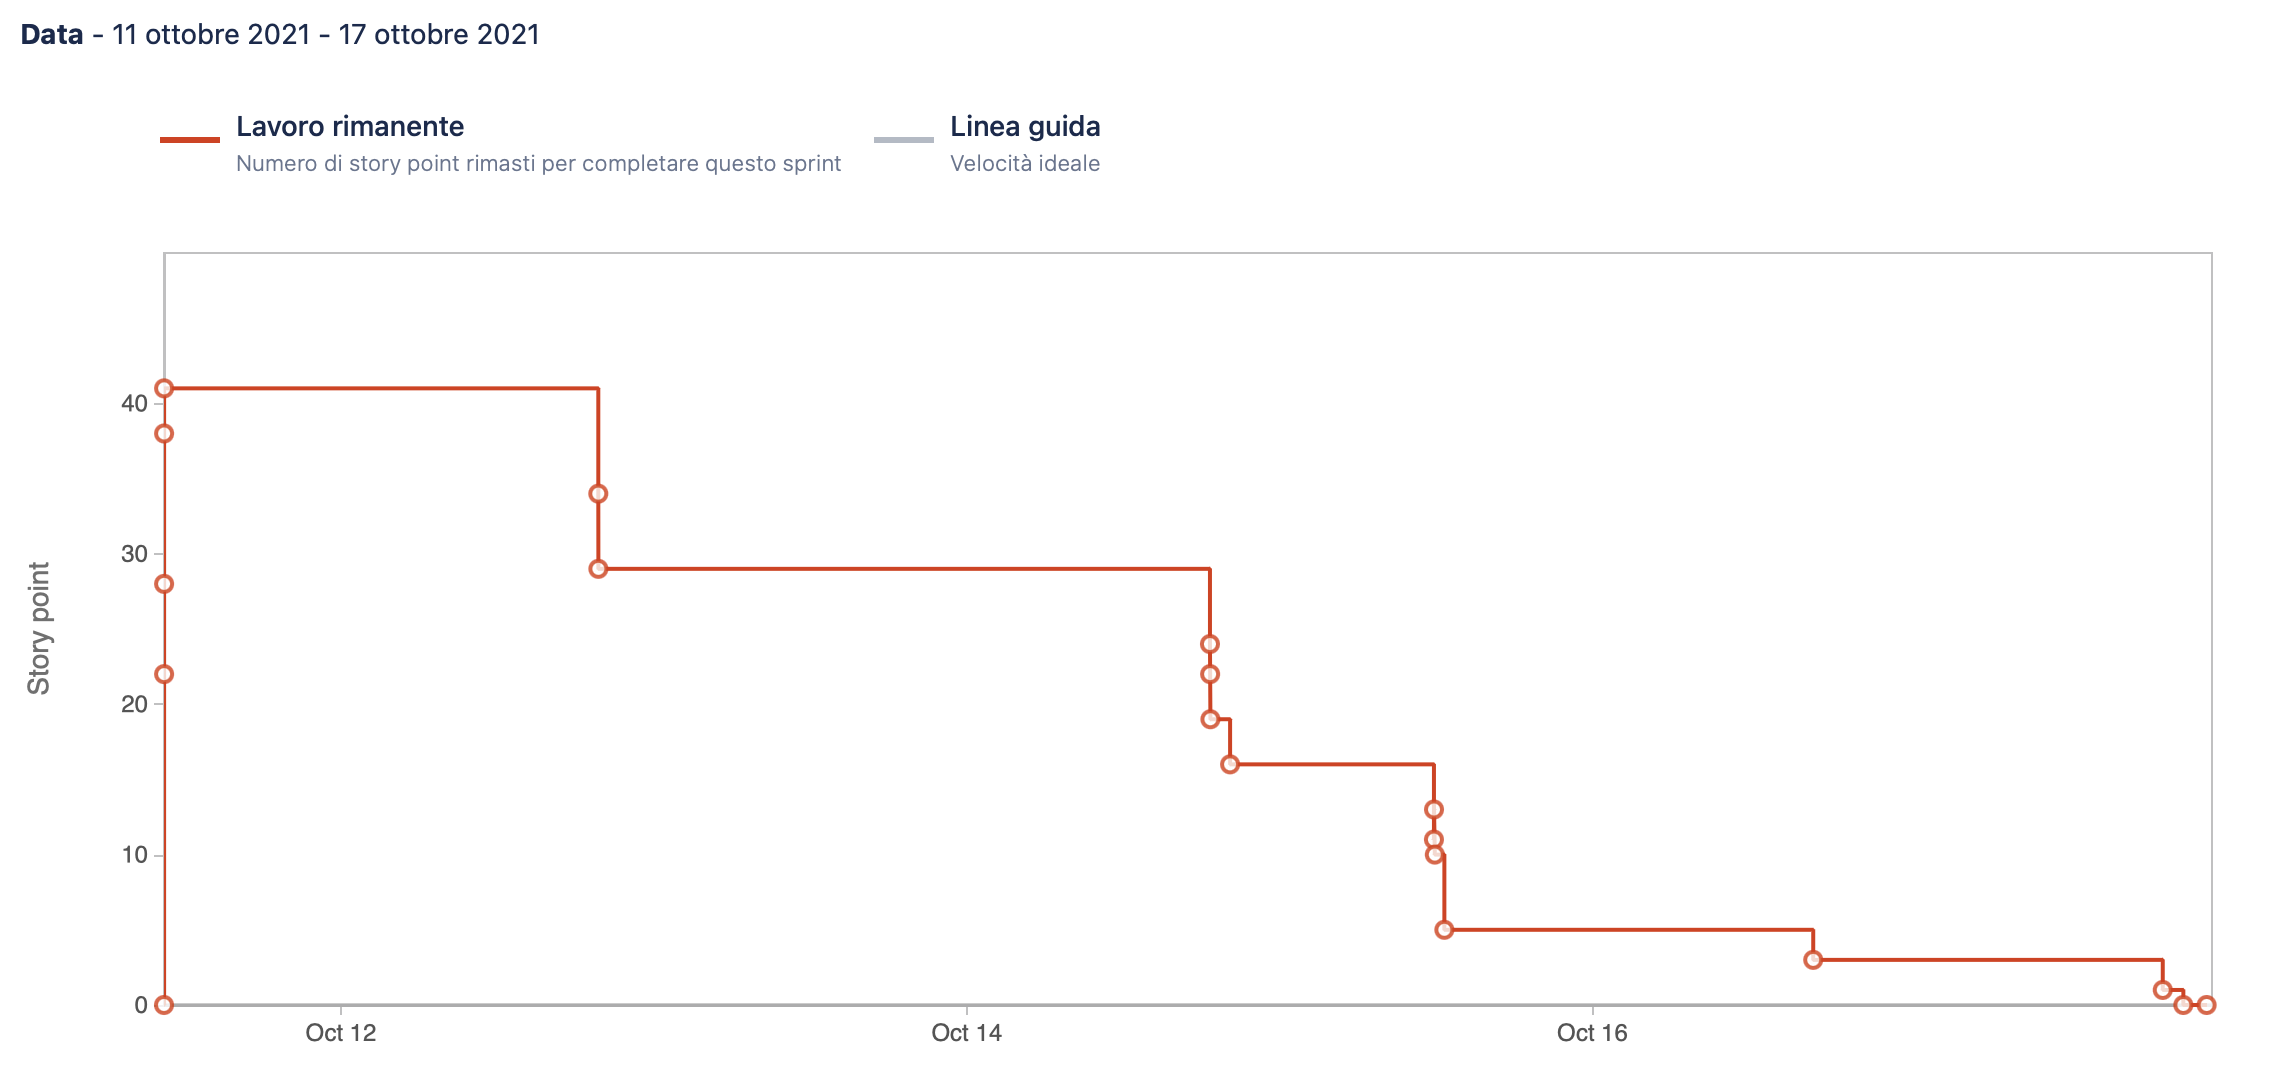
\includegraphics[scale=0.4]{sprint-3-burn-down.png}
    \caption{\textit{Grafico Burn-down primo sprint}} 
\end{figure}


\subsection{Sprint 4 18/10 - 24/10}
Il quarto sprint è stato incentrato principalmente sul dungeon e sulla feature dello sparo per il personaggio controllato dall'utente. 
In particolare, per quanto riguarda il dungeon, è stata implementata la generazione tramite prolog e, inoltre, la possibilità di navigare tra le stanze attraverso l'uso di porte. 
Essendo Indigo basato su Scala.js abbiamo integrato un engine Prolog scritto in javascript e creato un'interfaccia in Scala per interagirvi.

Nella prossima sprint, sarà necessario un refactor e una forte integrazione tra le parti sviluppate individualmente dai diversi componenti del team.

\begin{figure}[!hbt]
    \centering
    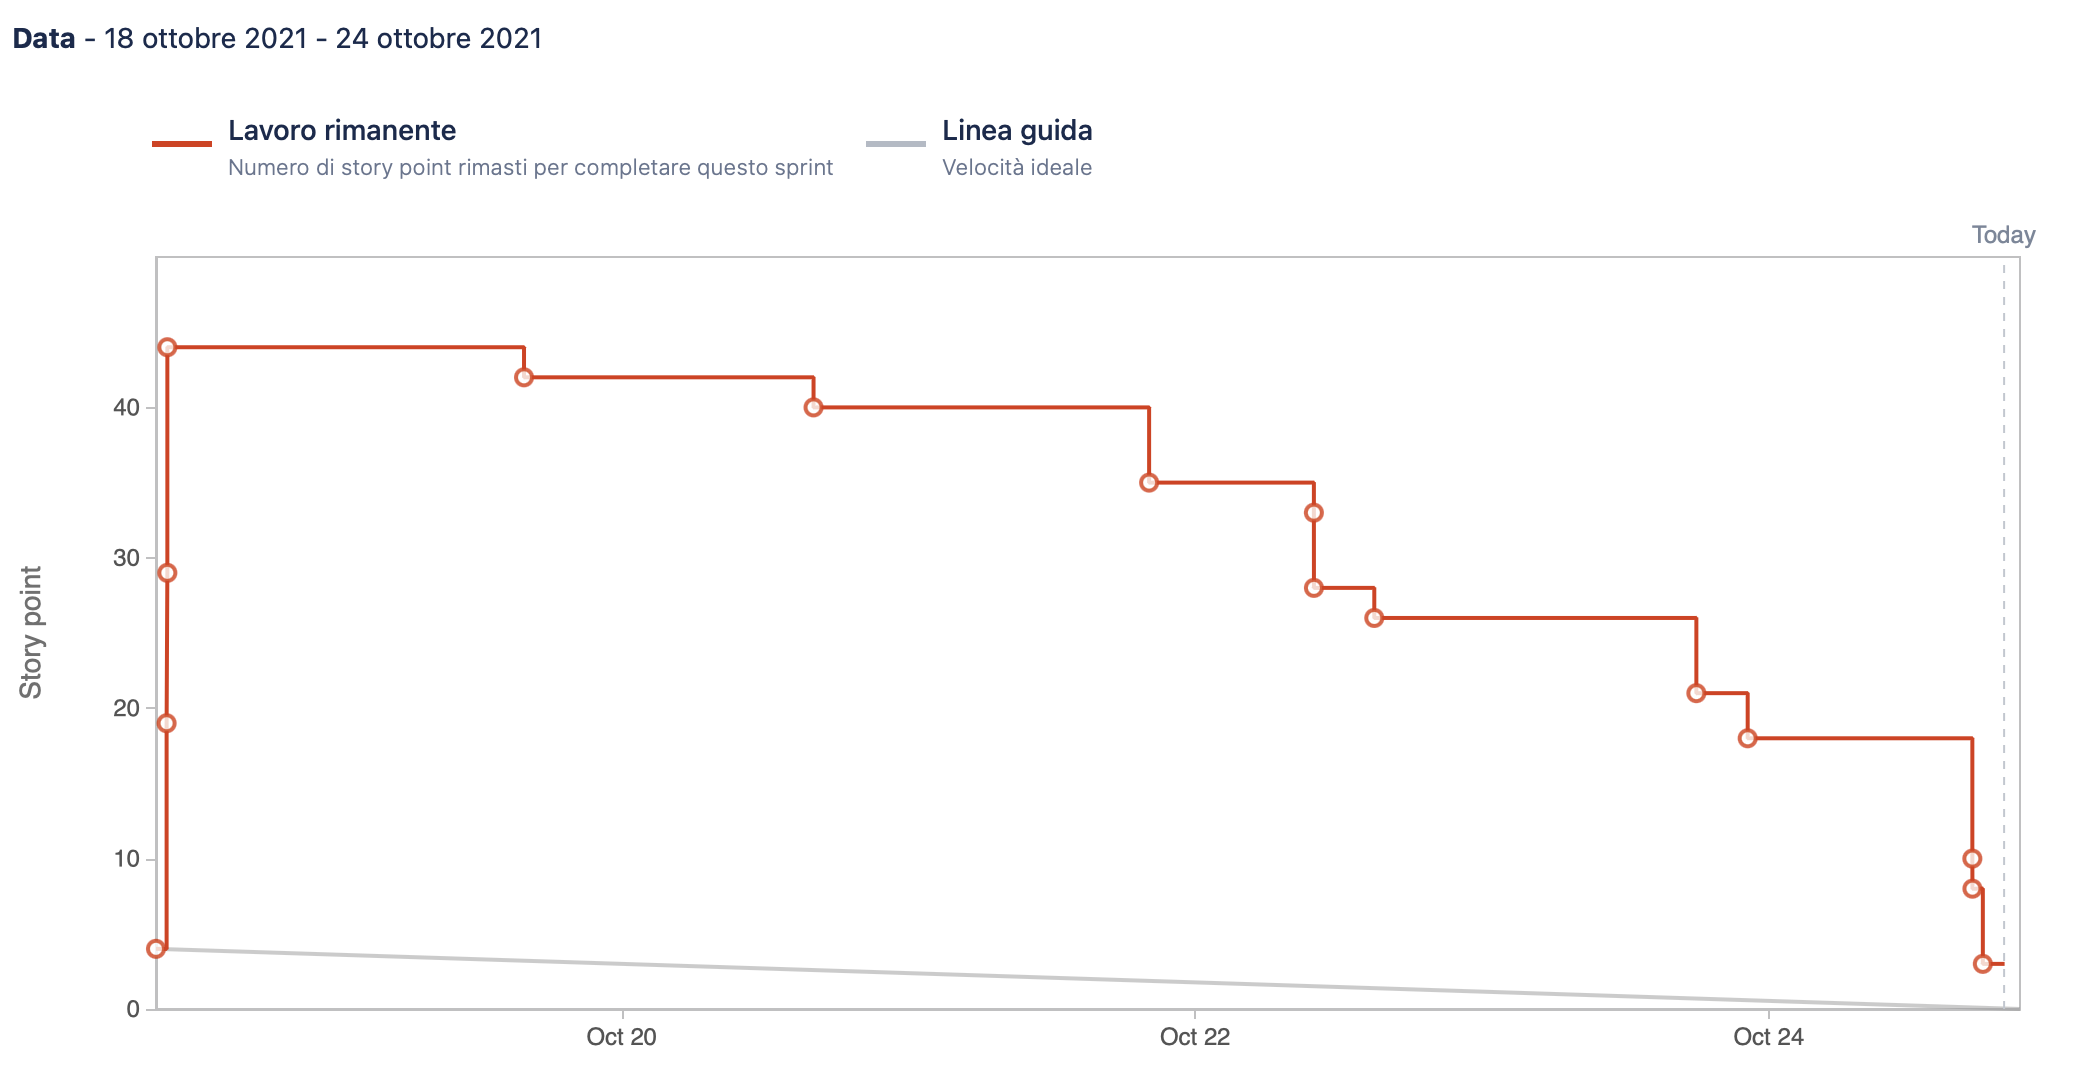
\includegraphics[scale=0.4]{sprint-4-burn-down.png}
    \caption{\textit{Grafico Burn-down primo sprint}} 
\end{figure}

\subsection{Sprint 5}

\subsection{Sprint 6}

\bibliographystyle{plain}

\end{document}